\documentclass{beamer}
\usepackage{graphicx}
%\usepackage{subfig}
\usepackage{multicol}
\usepackage{multimedia}
\usepackage{empheq}
\usepackage{lipsum} 
\usepackage{color}
\usepackage{comment}
\usepackage{bm}
%\usepackage{graphicx}
\usepackage{setspace}
\usepackage{float}
%\usepackage{lineno}
%\usepackage{verbatim}
\usepackage{amsmath}
\usepackage{amsfonts}
\usepackage{caption}
\usepackage{subcaption}

%\usepackage{movie9}
%\usepackage{subfig}
\usecolortheme[named=red]{structure}
\mode<presentation> {

% The Beamer class comes with a number of default slide themes
% which change the colors and layouts of slides. Below this is a list
% of all the themes, uncomment each in turn to see what they look like.

%\usetheme{default}
%\usetheme{AnnArbor}
%\usetheme{Antibes}
%\usetheme{Bergen}
%\usetheme{Berkeley}
%\usetheme{Berlin}
%\usetheme{Boadilla} maybe
\usetheme{CambridgeUS} 
%\usetheme{Copenhagen}
%\usetheme{Darmstadt}
%\usetheme{Dresden}
%\usetheme{Frankfurt}
%\usetheme{Goettingen}
%\usetheme{Hannover}
%\usetheme{Ilmenau}
%\usetheme{JuanLesPins}
%\usetheme{Luebeck}
%\usetheme{Madrid}
%\usetheme{Malmoe}
%\usetheme{Marburg}
%\usetheme{Montpellier}
%\usetheme{PaloAlto}
%\usetheme{Pittsburgh}
%\usetheme{Rochester}
%\usetheme{Singapore}
%\usetheme{Szeged}
%\usetheme{Warsaw}

% As well as themes, the Beamer class has a number of color themes
% for any slide theme. Uncomment each of these in turn to see how it
% changes the colors of your current slide theme.

%\usecolortheme{albatross}
%\usecolortheme{beaver}
%\usecolortheme{beetle}
%\usecolortheme{crane}
%\usecolortheme{dolphin}
%\usecolortheme{dove}
%\usecolortheme{fly}
%\usecolortheme{lily}
%\usecolortheme{orchid}
%\usecolortheme{rose}
%\usecolortheme{seagull}
%\usecolortheme{seahorse}
%\usecolortheme{whale}
%\usecolortheme{wolverine}


%\setbeamertemplate{footline} % To remove the footer line in all slides uncomment this line
%\setbeamertemplate{footline}[page number] % To replace the footer line in all slides with a simple slide count uncomment this line

%\setbeamertemplate{navigation symbols}{} % To remove the navigation symbols from the bottom of all slides uncomment this line
}

\usepackage{graphicx} % Allows including images
\usepackage{booktabs} % Allows the use of \toprule, \midrule and \bottomrule in tables
\usepackage{appendixnumberbeamer}
%----------------------------------------------------------------------------------------
%	TITLE PAGE
%----------------------------------------------------------------------------------------

\title[GAMs]{Generalized Additive Models: \\ Allowing for some wiggle room in your models
} % The short title appears at the bottom of every slide, the full title is only on the title page

\author[@sastoudt]{Sara Stoudt
} % Your name
\institute[Smith College] % Your institution as it will appear on the bottom of every slide, may be shorthand to save space
{
%\large{Smith College}\\ % Your institution for the title page
%%\medskip
%\textit{john@smith.com} % Your email address
}
\setbeamertemplate{navigation symbols}{}
\date{March 17, 2021} % Date, can be changed to a custom date

\begin{document}


\begin{frame}
\titlepage % Print the title page as the first slide

\end{frame}


\begin{frame}
\frametitle{About Me}
\begin{itemize}
\item currently teaching in the Statistical and Data Sciences Program at Smith College
\item PhD in Statistics at Berkeley
\begin{itemize}
\item ecology: evaluating fitness for purpose of a variety of data collection protocols for species distribution and abundance models
\item ecology: evaluating model fit in terms of community metrics for joint species distribution models
\item statistics communication: co-authored a book \textit{Communicating with Data: The Art of Writing for Data Science} with Deborah Nolan
\end{itemize}
\end{itemize}

Materials here: \url{https://github.com/sastoudt/MZES_GAMs}

\end{frame}


\begin{frame}
\frametitle{GAMs in my work}


\begin{figure}
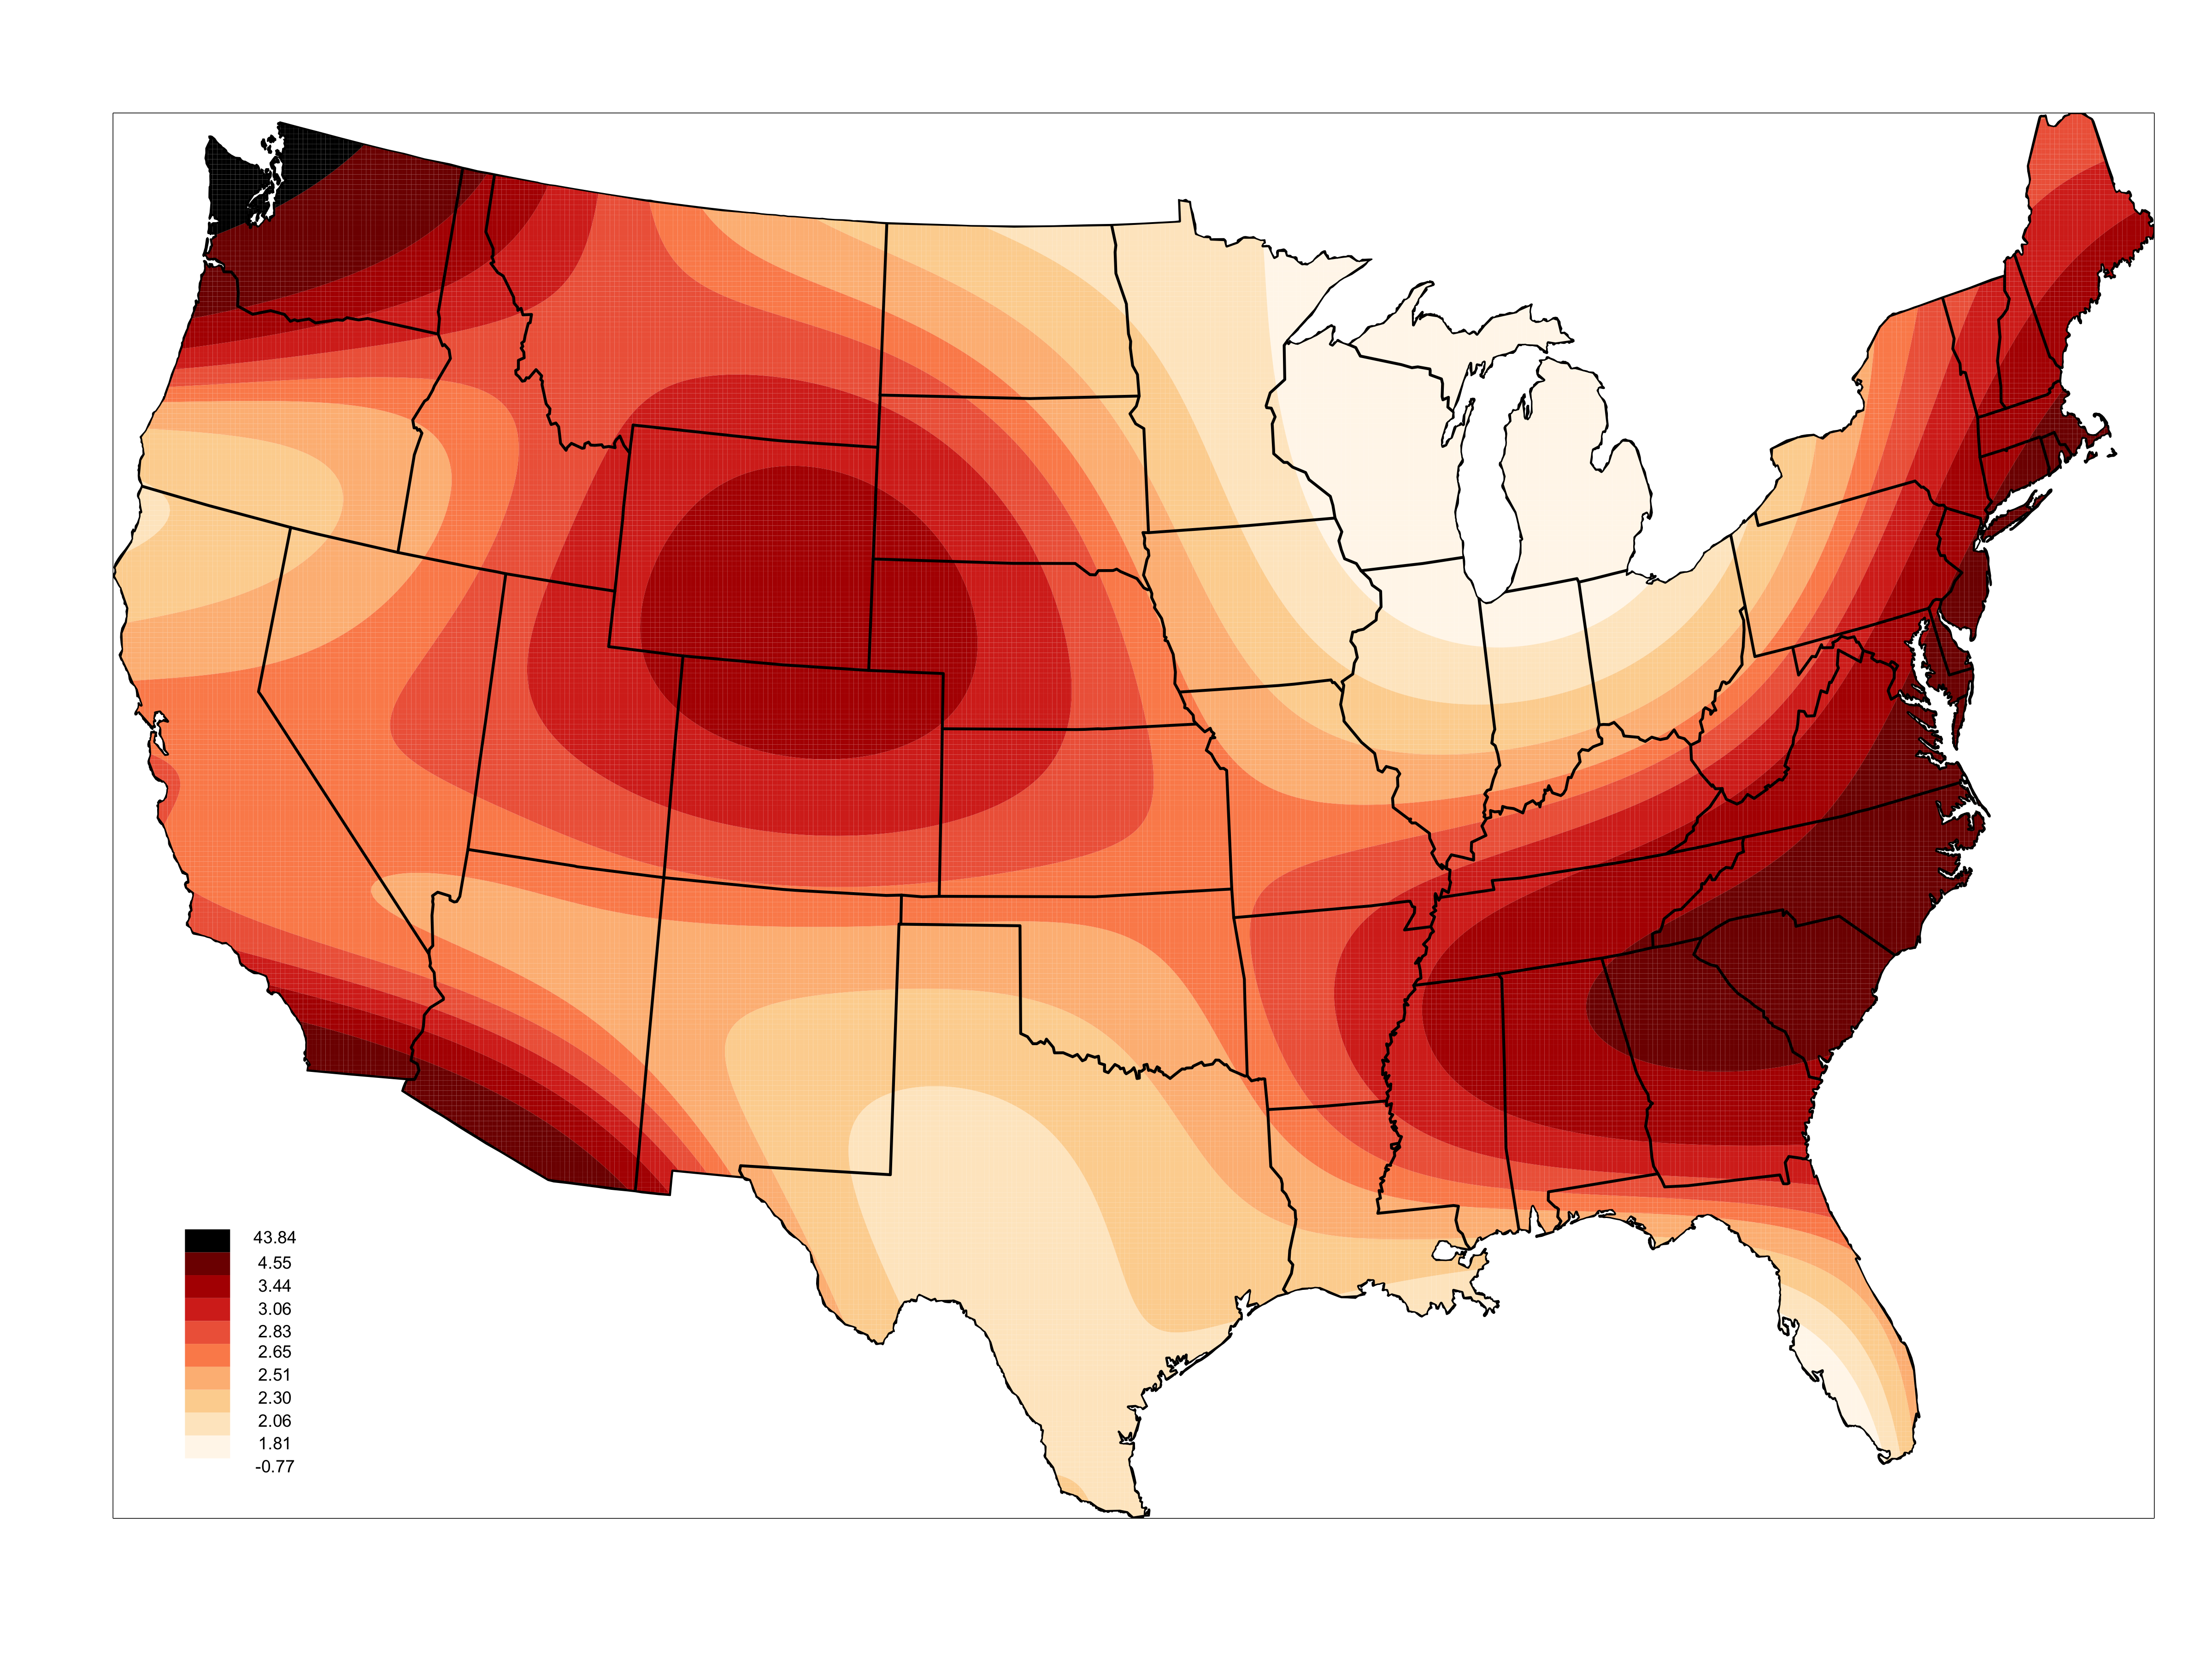
\includegraphics[scale=.02]{figures/gamTE3BestNice}
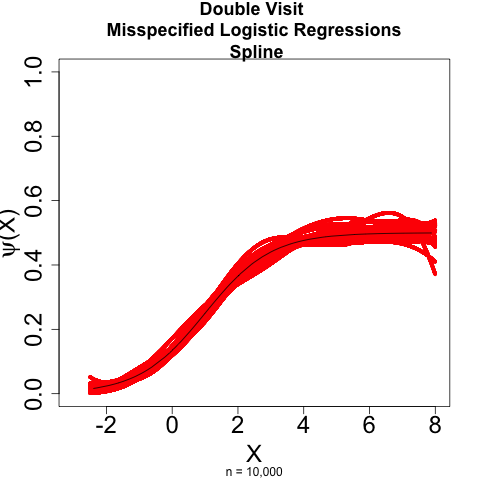
\includegraphics[scale=.2]{figures/logregSplineMisspecifiedExpandRangeDVPsi}


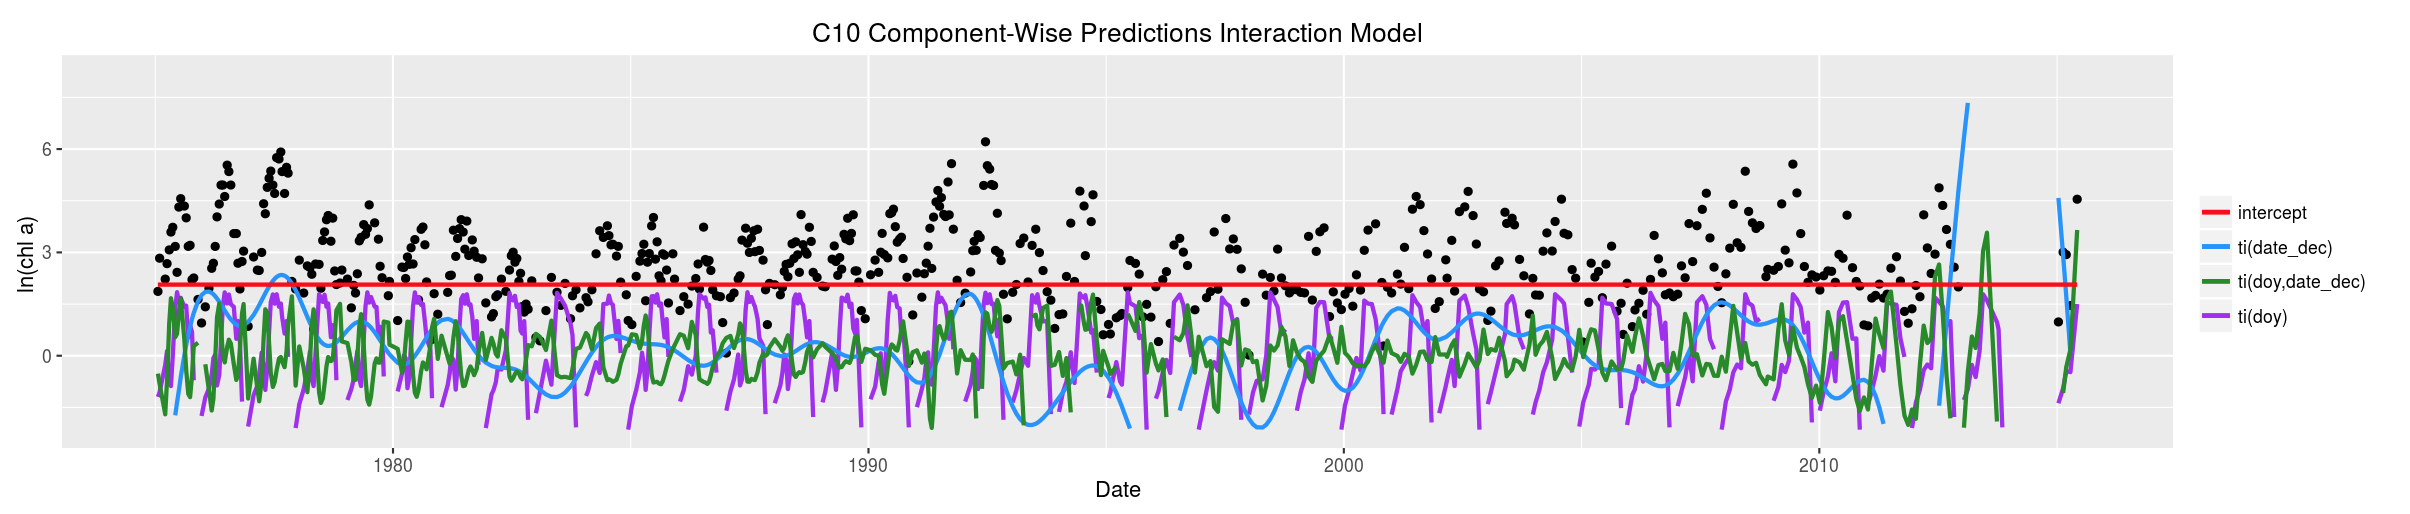
\includegraphics[scale = .2]{figures/sfeiGAM1}
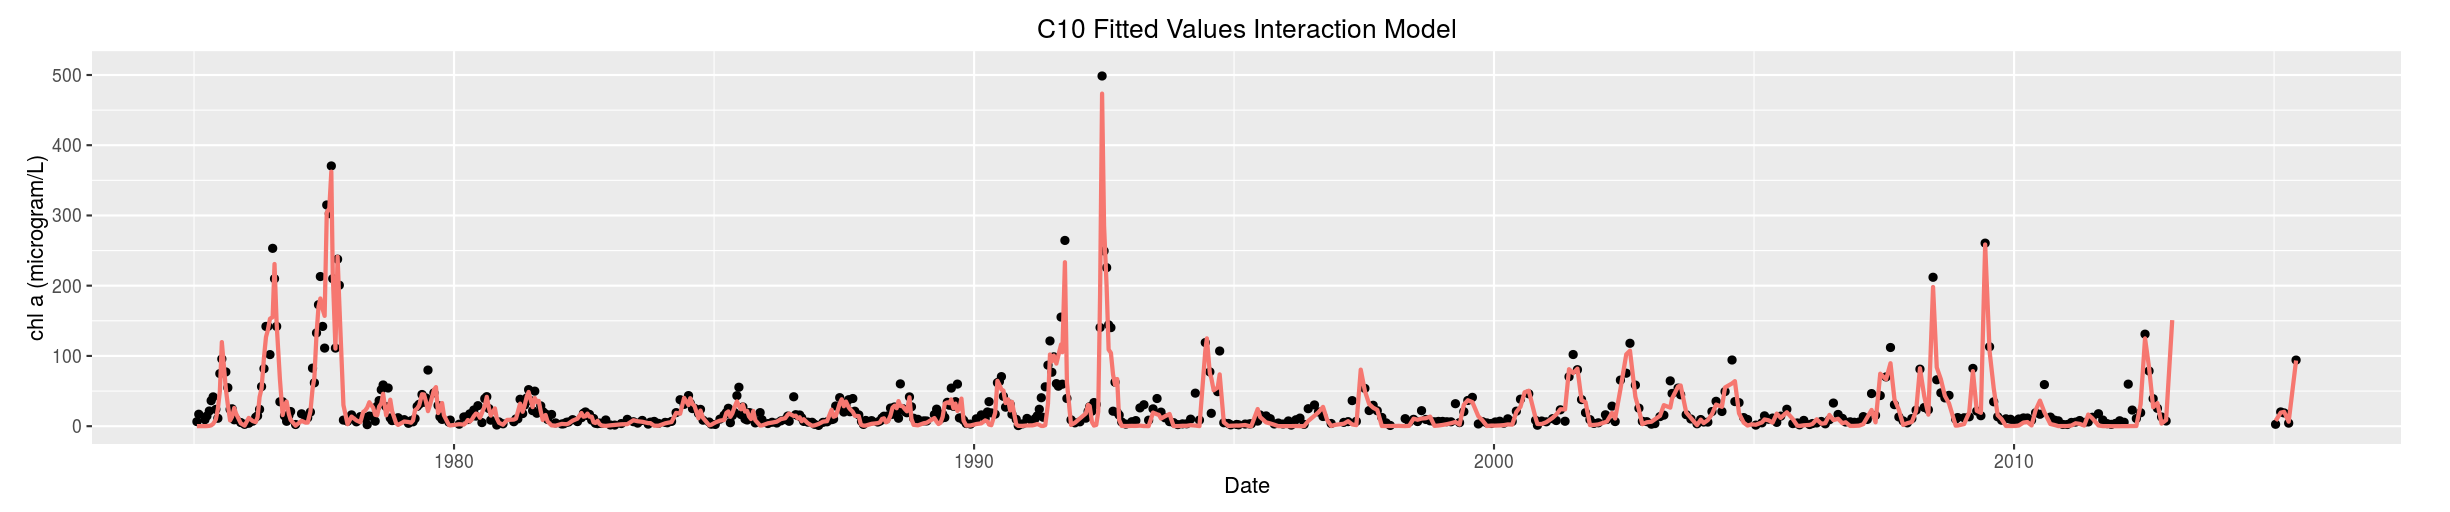
\includegraphics[scale=.2]{figures/sfeiGAM2}

\end{figure}

\end{frame}

\begin{frame}
\frametitle{Setting the Scene}


\begin{multicols}{2}

\begin{figure}
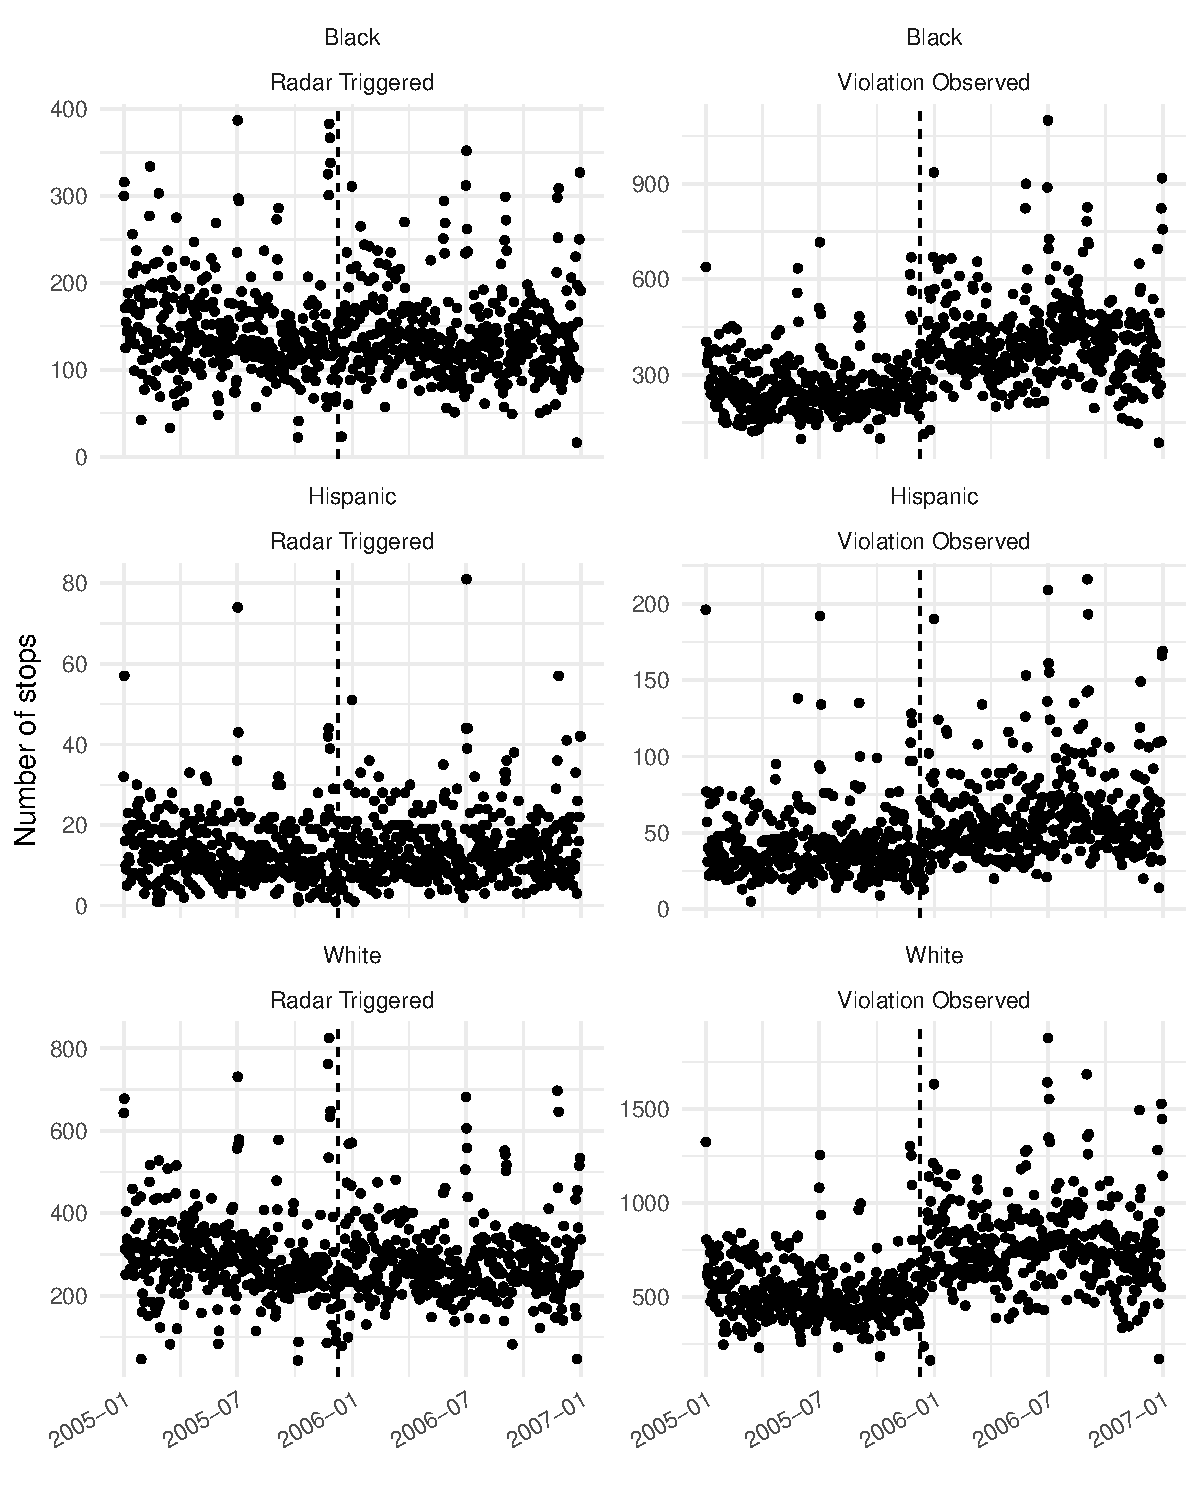
\includegraphics[scale=.25]{figures/stopData}
\end{figure}

\columnbreak

\begin{itemize}

\item ``Using change in a seat belt law to study racially-biased policing in South Carolina" by Corinne A Riddell, Jay S Kaufman, Jacqueline M Torres, and Sam Harper

\item \url{https://github.com/corinne-riddell/SCarolinaTrafficStops}

\end{itemize}
\end{multicols}


\end{frame}





\begin{frame}
\frametitle{Linear Model - \texttt{lm}}

\begin{multicols}{2}

$$ Y = X\beta +  \epsilon $$

$$\text{daily number of stops} \sim \beta_{driverRace} + $$
$$\beta_{isPostPolicy}+ \beta_{driverRace, isPostPolicy}+$$
$$ \beta_{dayOfWeek} + \beta*\text{month} $$

Choices:

\begin{itemize}
\item which covariates $X$ to use
\end{itemize}

\columnbreak

\begin{figure}
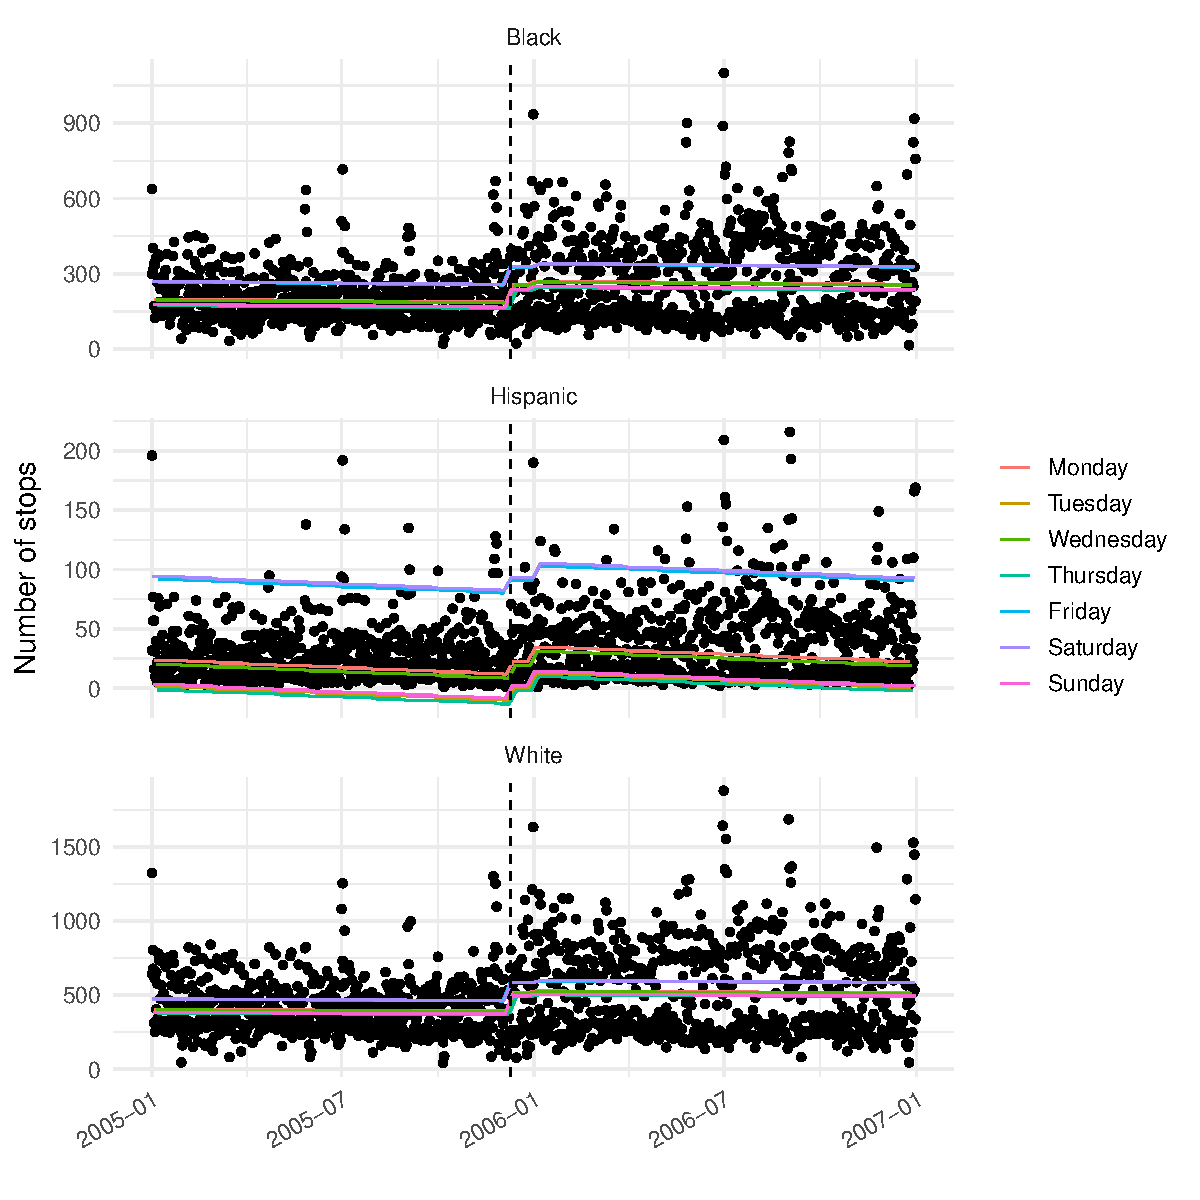
\includegraphics[scale=.3]{figures/lmResults}
\end{figure}

\end{multicols}


\end{frame}

\begin{frame}
\frametitle{Generalized Linear Model - \texttt{glm}}

\begin{multicols}{2}

$$ E[Y] \sim g^{-1}(X\beta) $$
$$ g(E[Y]) \sim X\beta $$

$$g(\text{daily number of stops}) \sim \beta_{driverRace} + $$
$$\beta_{isPostPolicy}+ \beta_{driverRace, isPostPolicy}+$$
$$ \beta_{dayOfWeek} + \beta*\text{month} $$


Choices:

\begin{itemize}
\item which covariates $X$ to use
\item response distribution (\texttt{quasipoisson}) and link function $g$
\end{itemize}

\columnbreak

\begin{figure}
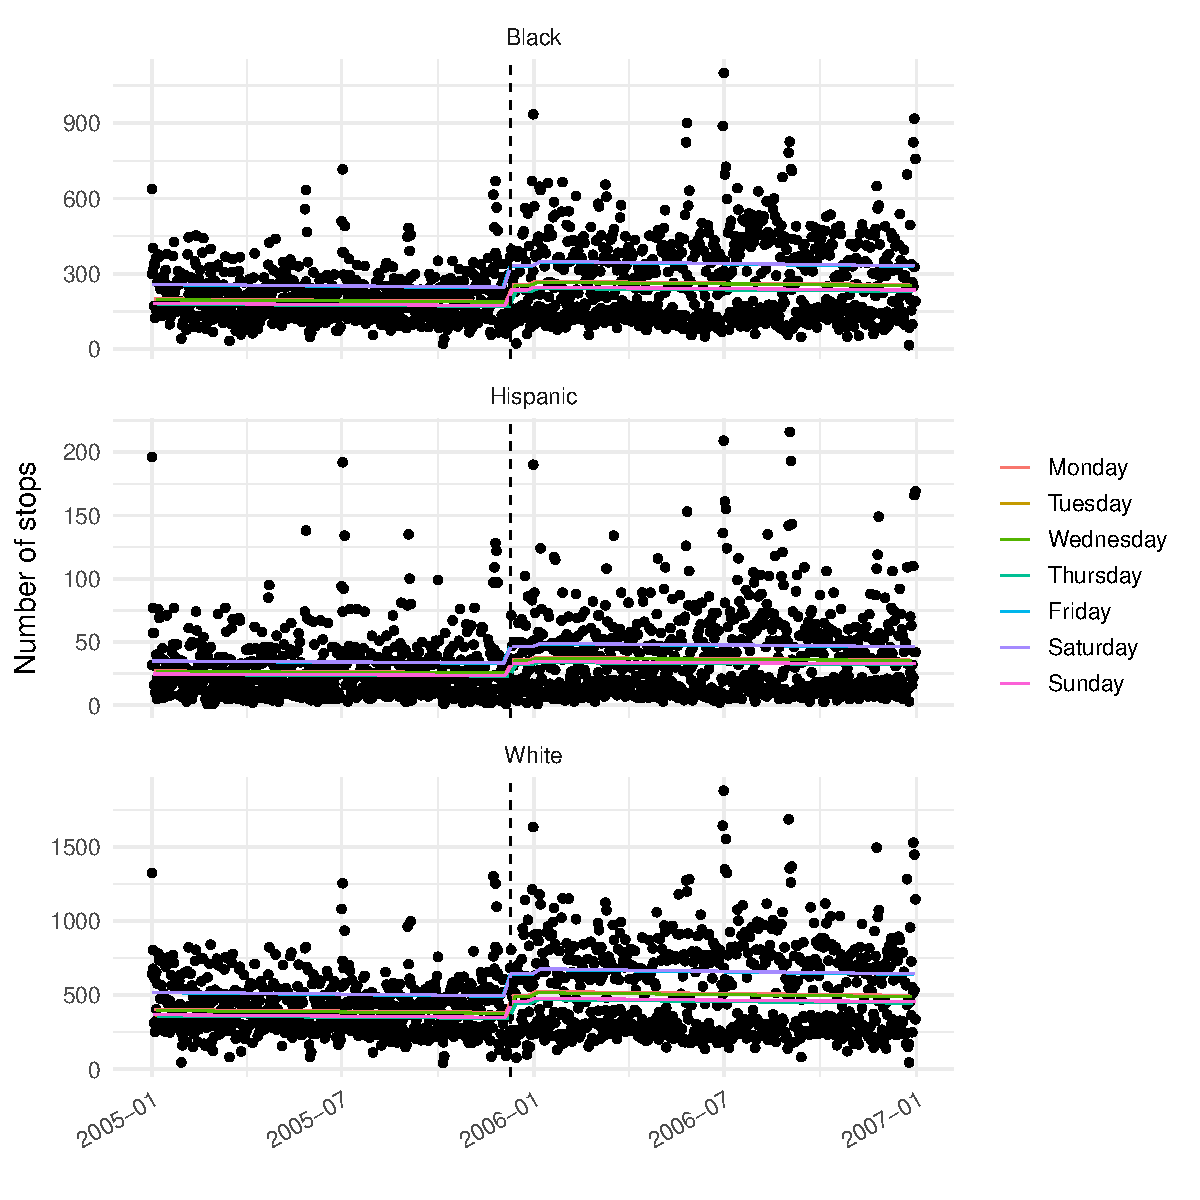
\includegraphics[scale=.3]{figures/glmResults}
\end{figure}

\end{multicols}


\end{frame}

\begin{frame}
% Generalized additive models allow us to use information that we have about the distribution of the response. A generalized additive model relaxes the assumption of normality in the response variable, allows for the response variable to follow distributions other than the normal distribution, and is specified as a sum of smooth functions of predictor variables.

%A link function maps the linear term $\textbf{X}_i\beta$ in a GLM to the expected value of the response variable $y_i$ so that $g(\mu_i)$ has a range of $[-\infty,\infty]$ as desired.

\frametitle{Generalized Additive Models: Intuition}

$$ g(E[Y]) = X\beta + f_1(x_{1i})+f_2(x_{2i})$$

$$g(\text{daily number of stops}) \sim \beta_{driverRace} + $$
$$\beta_{isPostPolicy}+ \beta_{driverRace, isPostPolicy}+$$
$$ f_1(\text{dayOfWeek}) + f_2(\text{month}) $$


Choices: 
\begin{itemize}
\item which covariates $X$ to use
\item response distribution and link function $g$
\item type of basis that defines $f_i$
\item dimension of basis
\item smoothing parameter
\end{itemize}

\footnotesize{*Simon N. Wood. \textit{Generalized Additive Models: An Introduction with R.} Chapman and Hall/CRC, 2017.}
\end{frame}

\begin{frame}
\frametitle{GAM: Parameter Intuition}
\begin{figure}
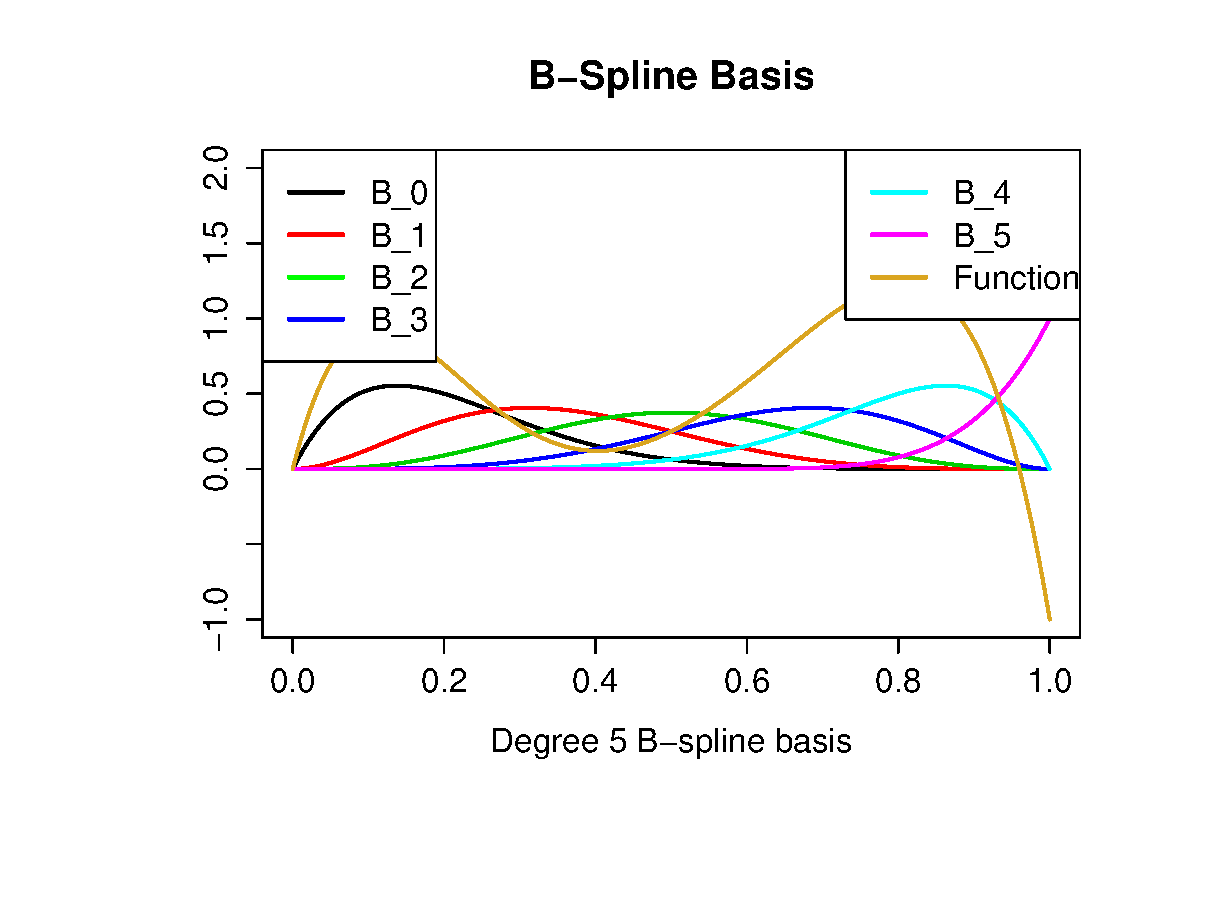
\includegraphics[scale=.4]{figures/bSplineBasis}
% others: cubic regression spline, thin plate regression spline
\end{figure}

\end{frame}





\begin{frame}
\frametitle{GAM: Parameter Intuition}
\begin{figure}

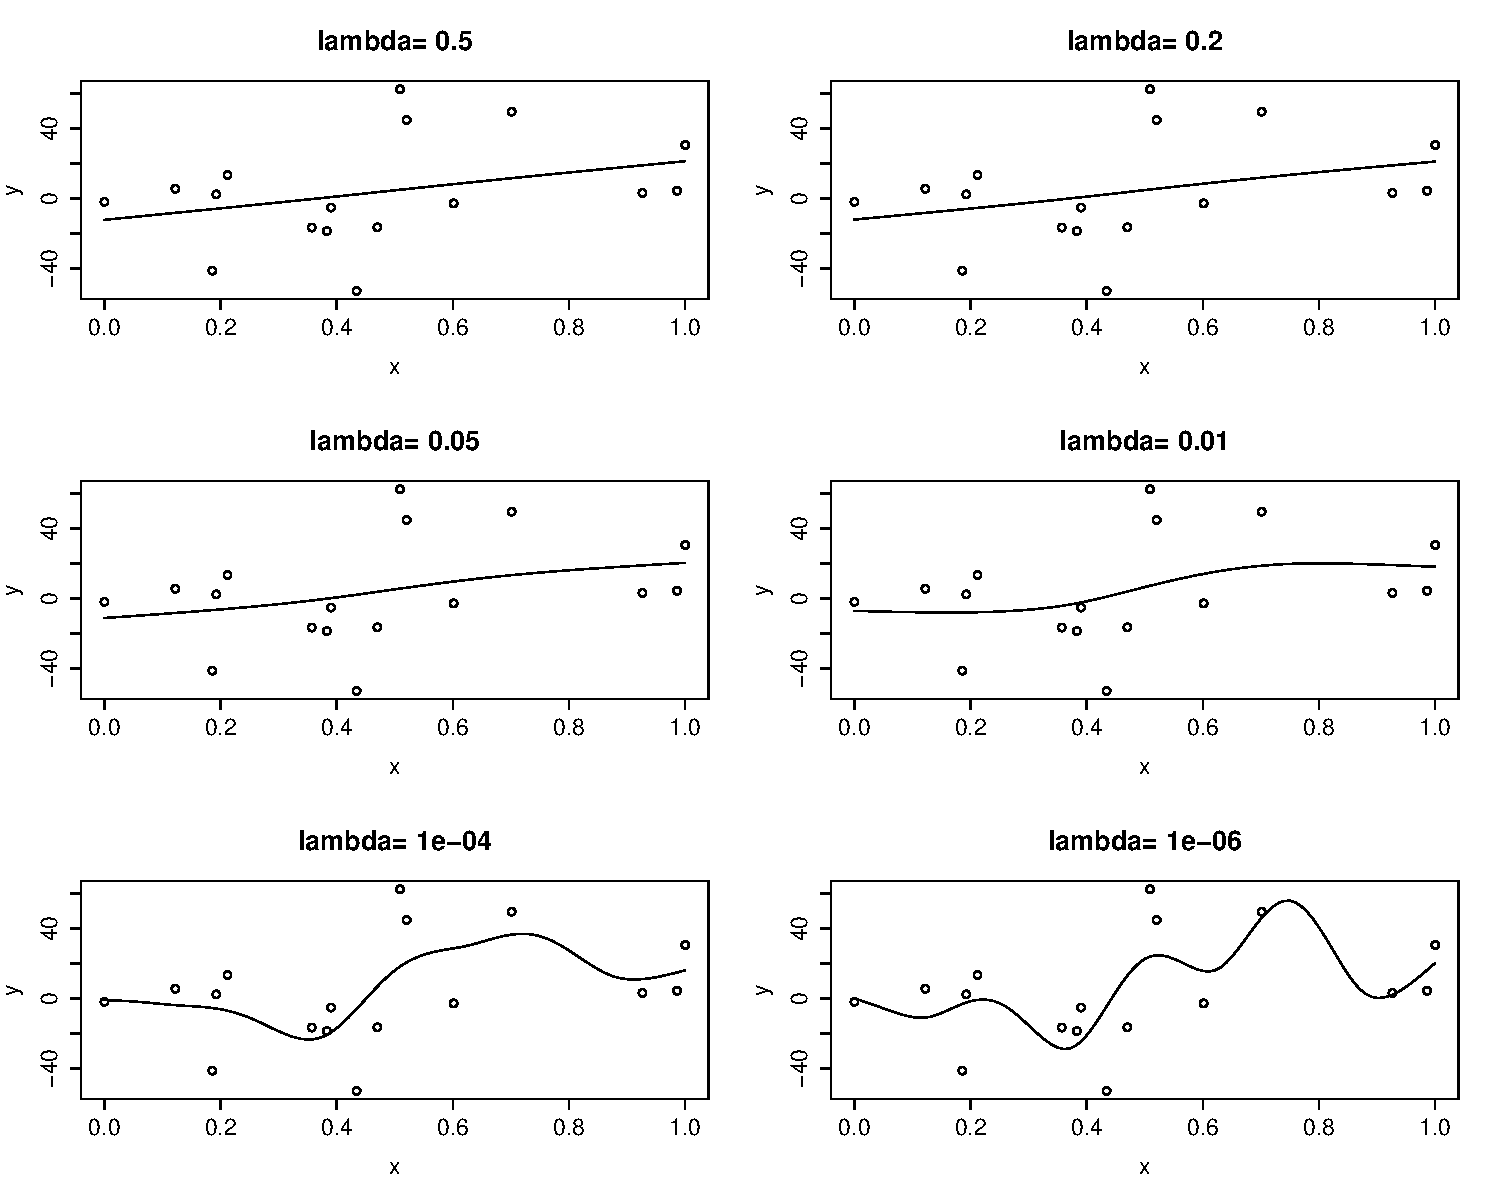
\includegraphics[scale=.35]{figures/splineDiffLambda}
% penalizes ``wiggliness"
\end{figure}
\end{frame}

\begin{frame}
\frametitle{Generalized Additive Model - \texttt{mgcv::gam}}

\begin{multicols}{2}
$$g(\text{daily number of stops}) \sim \beta_{driverRace} + $$
$$\beta_{isPostPolicy}+ \beta_{driverRace, isPostPolicy}+$$
$$ f_1(\text{dayOfWeek}) + f_2(\text{month}) $$

Choices:

\begin{itemize}
\item which covariates $X$ to use
\item response distribution (\texttt{quasipoisson}) and link function $g$
\item type of basis that defines $f_i$
\item dimension of basis
\item smoothing parameter (default: GCV)
\end{itemize}

\columnbreak

\begin{figure}
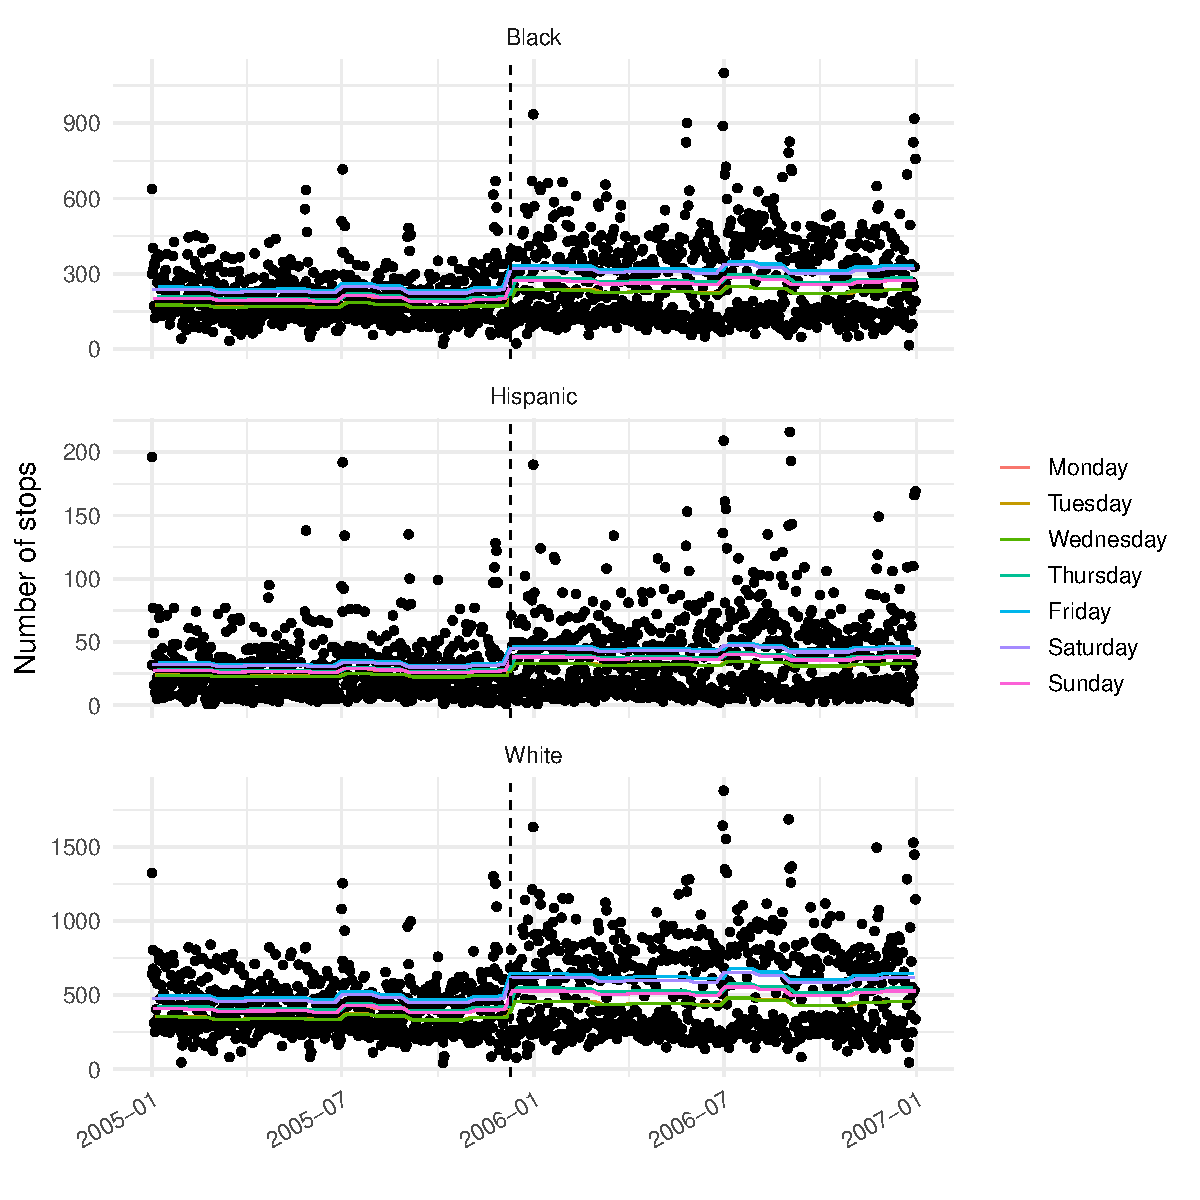
\includegraphics[scale=.3]{figures/gamResults}
\end{figure}

\end{multicols}


\end{frame}

\begin{frame}
\frametitle{Under the Hood - Cyclic Basis}

\texttt{s(month, bs = "cc")}

\begin{itemize}
\item constrained to have the same beginning and end
\item helpful for time components
\item when you aren't in the mood to do a formal time series analysis
\end{itemize}

\end{frame}

\begin{frame}
\frametitle{Under the Hood - Choosing $k$}

\begin{multicols}{2}
\texttt{$s(day\_of\_week\_num, bs = "cc", k = 4)$}

\begin{itemize}
\item $k$ controls the maximum amount of flexibility
\item bigger $k$ means more computational complexity
\item constrained by how much data you have (R will yell at you if you try to go too big)
\end{itemize}

\columnbreak

\texttt{gam.check(model)}

\begin{itemize}
\item there isn't one magic $k$, robust to choice of $k$ as long as in a reasonable range
\item but did I pick a $k$ big enough?
\item rough guide: small p-value means you could probably benefit from increasing $k$
\end{itemize}

\end{multicols}

\end{frame}

\begin{frame}
\frametitle{Under the Hood - Seeing the Smooths}
\begin{center}
\texttt{plot(model, rug = T)}
\end{center}

\begin{figure}
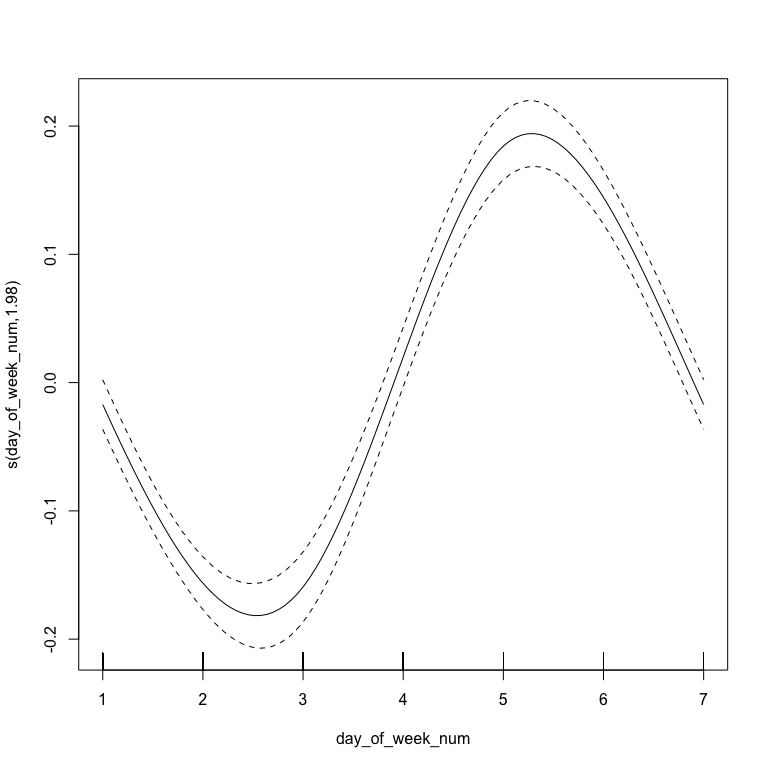
\includegraphics[scale=.2]{figures/exampleSmooth1}
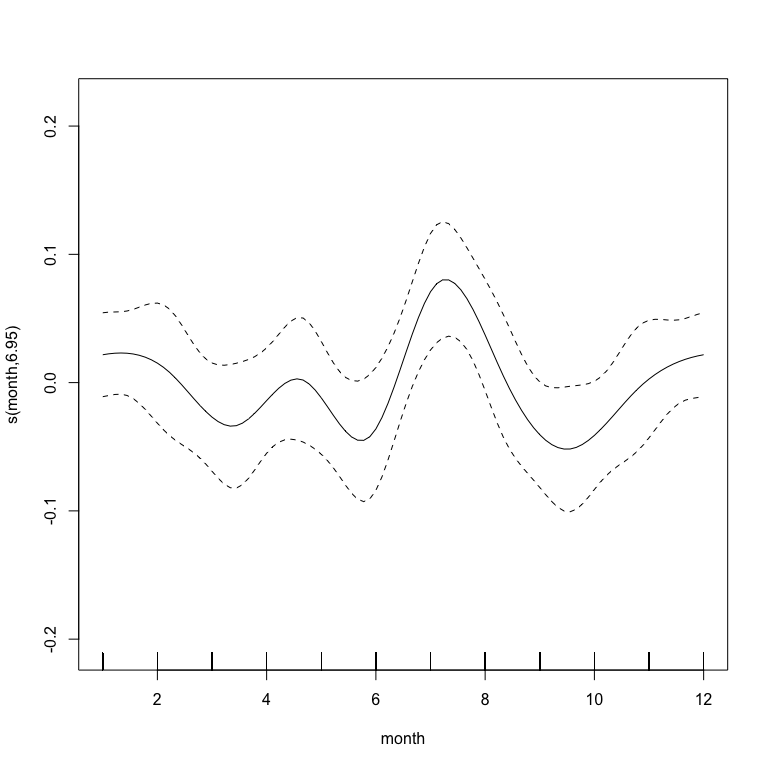
\includegraphics[scale=.2]{figures/exampleSmooth2}
\end{figure}


\end{frame}




\begin{frame}
\frametitle{Generalized Additive Model - \texttt{mgcv::gam}}

\begin{multicols}{2}
$$g(\text{daily number of stops}) \sim \beta_{driverRace} + $$
$$\beta_{isPostPolicy}+ \beta_{driverRace, isPostPolicy}+$$
$$ f_1(\text{dayOfWeek}) + f_2(\text{dayOfMonth})+ $$
$$ f_3(\text{dayOfYear})$$


\columnbreak

\begin{figure}
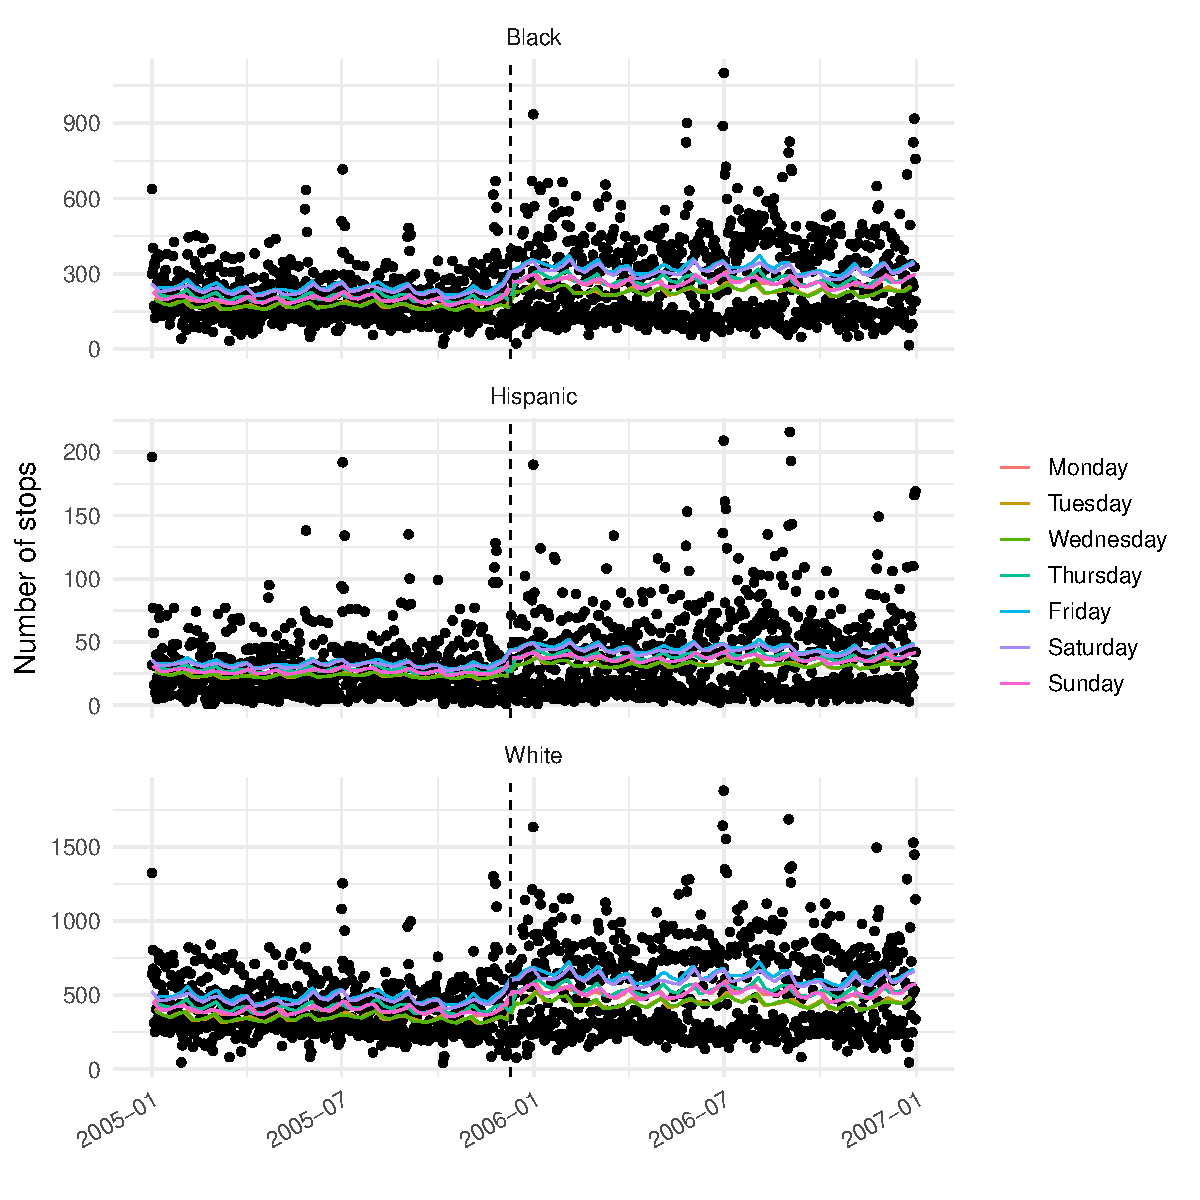
\includegraphics[scale=.3]{figures/gamResults2}
\end{figure}

\end{multicols}

\end{frame}

\begin{frame}
\frametitle{More Smooths}
\begin{center}
\texttt{plot(model, rug = T)}
\end{center}

\begin{figure}
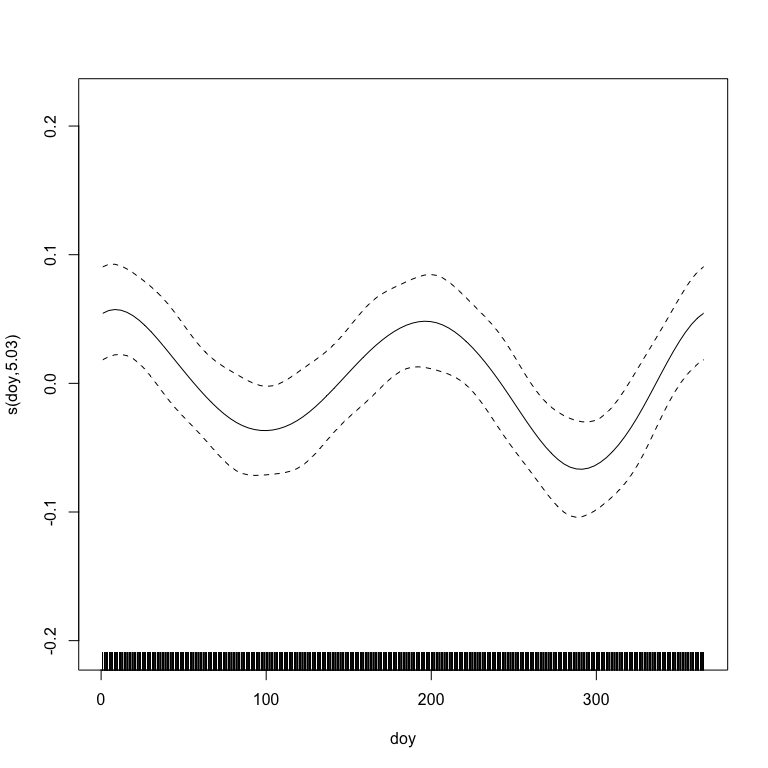
\includegraphics[scale=.2]{figures/exampleSmooth1b}
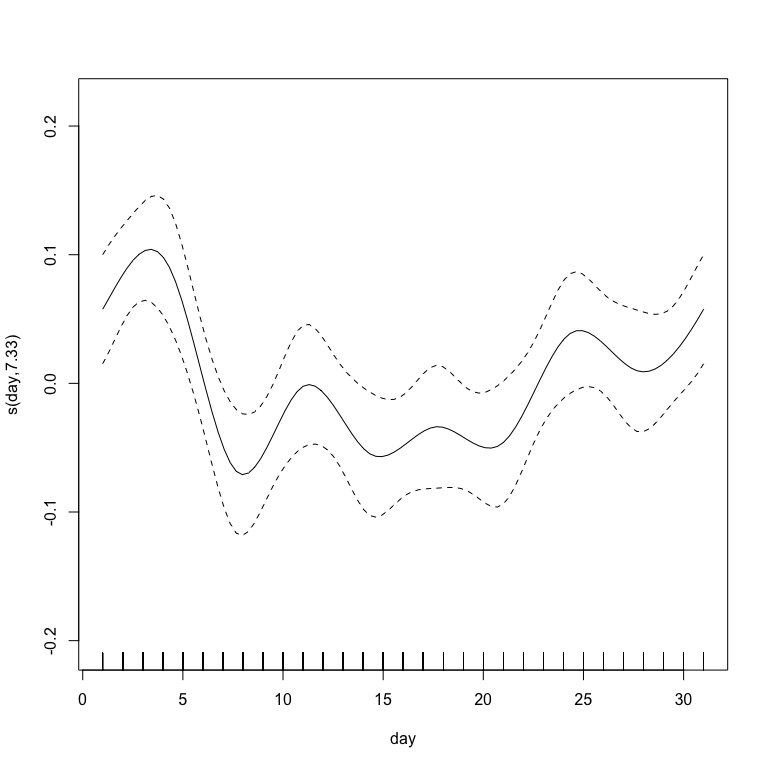
\includegraphics[scale=.2]{figures/exampleSmooth2b}
\end{figure}

Are these wiggles ``real"?

\end{frame}

\begin{frame}
\frametitle{Setting the Scene}


\begin{figure}
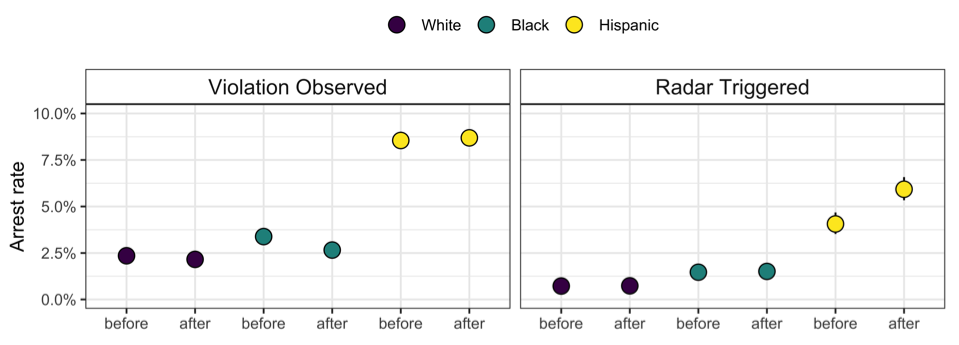
\includegraphics[scale=.5]{figures/arrestRates}
\end{figure}


\begin{itemize}

\item ``Using change in a seat belt law to study racially-biased policing in South Carolina" by Corinne A Riddell, Jay S Kaufman, Jacqueline M Torres, and Sam Harper

\item \url{https://github.com/corinne-riddell/SCarolinaTrafficStops}

\end{itemize}

\end{frame}

\begin{frame}
\frametitle{Big GAMs - \texttt{mgcv::bam}}


\begin{multicols}{2}
$$g(\text{arrest}) \sim \beta_{driverRace} + $$
$$ \beta_{gender} + f_1(\text{age}, bs = "cr") +$$
$$\beta_{isPostPolicy}+ \beta_{driverRace, isPostPolicy}$$


\begin{itemize}
\item response distribution (\texttt{binomial}) 
\item link function $g$ (\texttt{logit})
\end{itemize}

\columnbreak

\begin{figure}
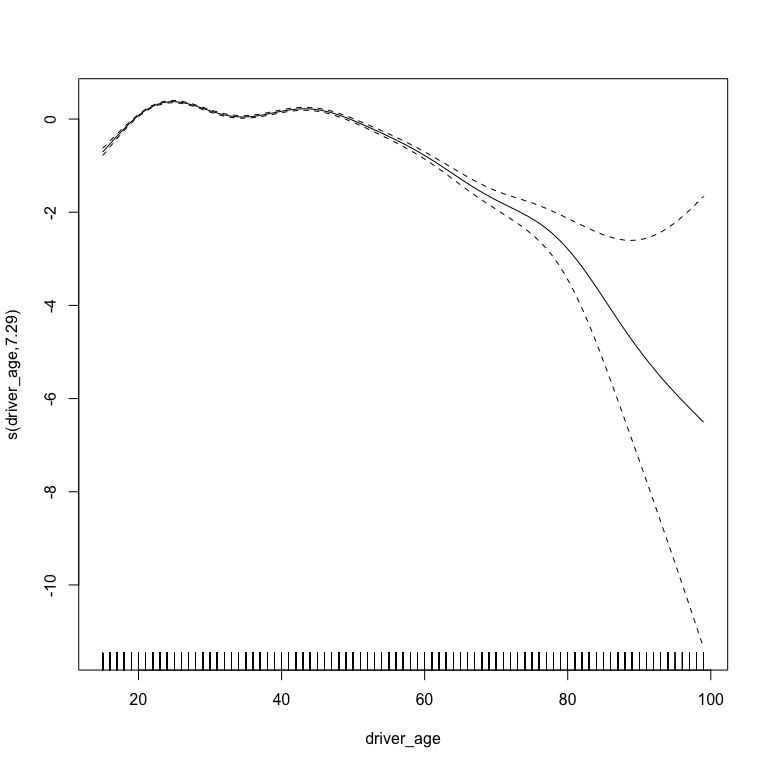
\includegraphics[scale=.2]{figures/smoothAge}
\end{figure}

\end{multicols}

\end{frame}

\begin{frame}
\frametitle{Shrinkage Splines - \texttt{bs = "cs"}}


\begin{multicols}{2}
$$g(\text{arrest}) \sim \beta_{driverRace} + $$
$$ \beta_{gender} + f_1(\text{age}) +$$
$$\beta_{isPostPolicy}+ \beta_{driverRace, isPostPolicy}+$$
$$ f_1(\text{dayOfWeek}) + f_2(\text{dayOfMonth})+ $$
$$ f_3(\text{dayOfYear})$$


\begin{itemize}
\item response distribution (\texttt{binomial}) 
\item link function $g$ (\texttt{logit})
\end{itemize}

\columnbreak

\begin{figure}
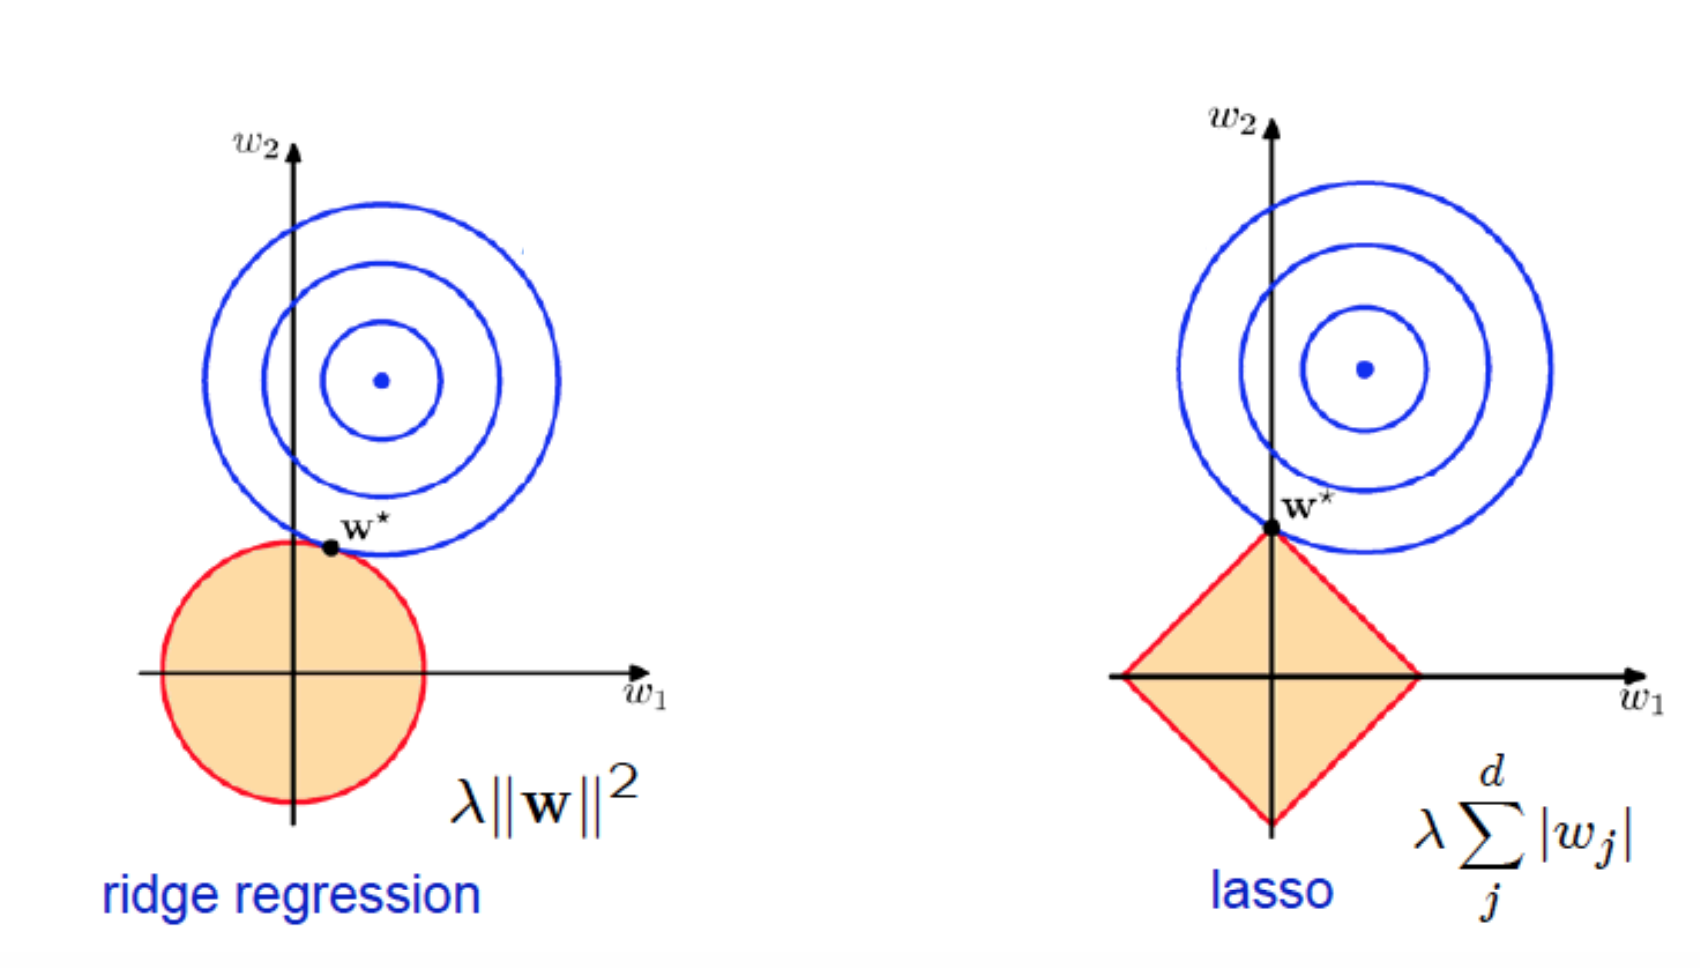
\includegraphics[scale=.2]{figures/regularizationEx}
\end{figure}

\footnotesize{Figure credit: \url{http://alex.smola.org/teaching/cmu2013-10-701/slides/13_recitation_lasso.pdf}}

\end{multicols}

\end{frame}

\begin{frame}
\frametitle{Real wiggles?}

\begin{figure}
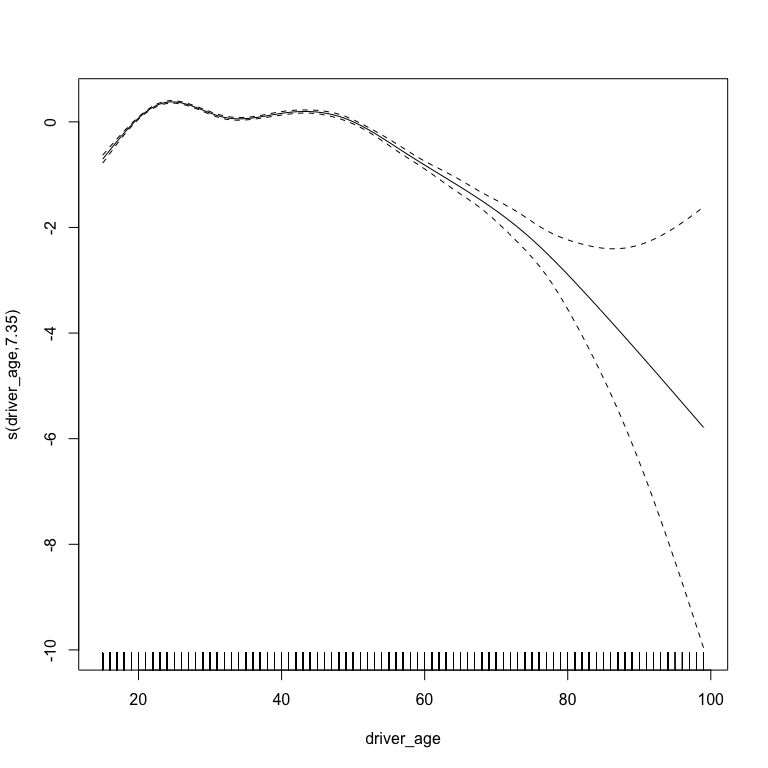
\includegraphics[scale=.13]{figures/og1}
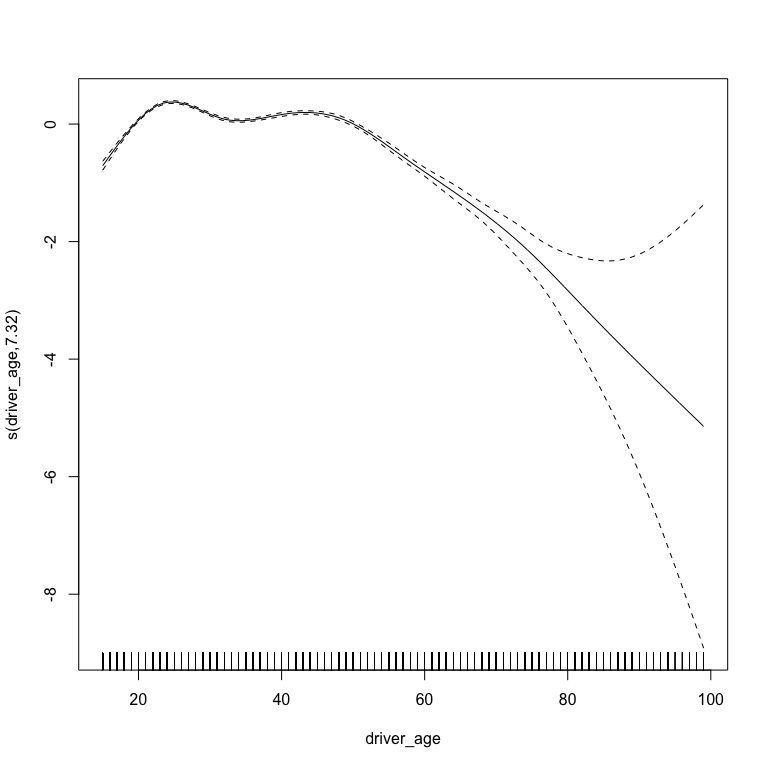
\includegraphics[scale=.13]{figures/shrinkage1}

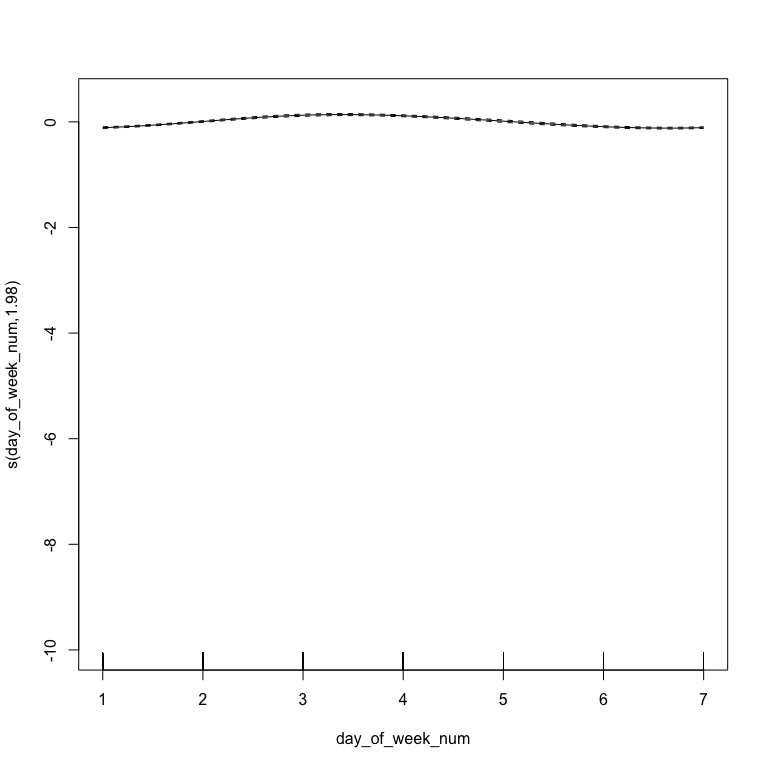
\includegraphics[scale=.13]{figures/og4}
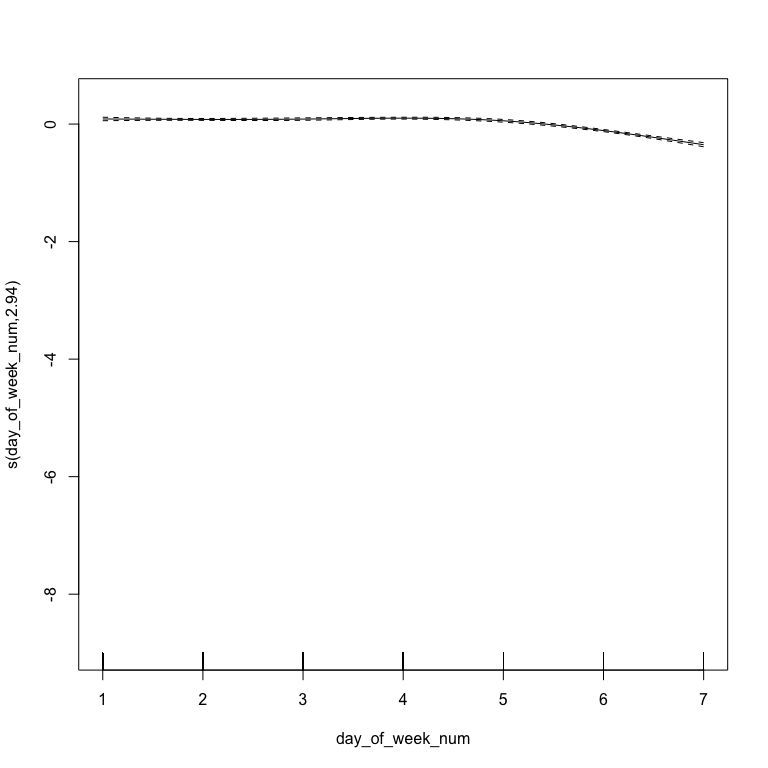
\includegraphics[scale=.13]{figures/shrinkage4}
\end{figure}

\end{frame}


\begin{frame}
\frametitle{Subtle shrinkage happening...}

\begin{figure}
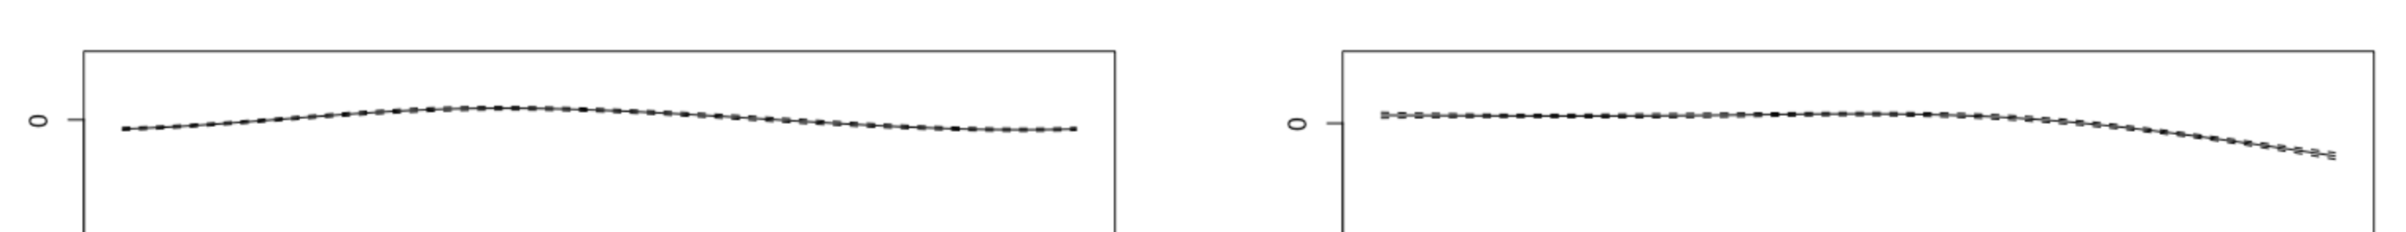
\includegraphics[scale=.28]{figures/zoomIn}
\end{figure}

\end{frame}



\begin{frame}
\frametitle{Multidimensional Smoothing}

\begin{multicols}{2}
\texttt{te(lon, lat)}

\begin{itemize}
\item two-dimensional smooth
\item helpful for spatial components
\item when you aren't in the mood to do a formal spatial analysis
\end{itemize}

\columnbreak

\begin{figure}
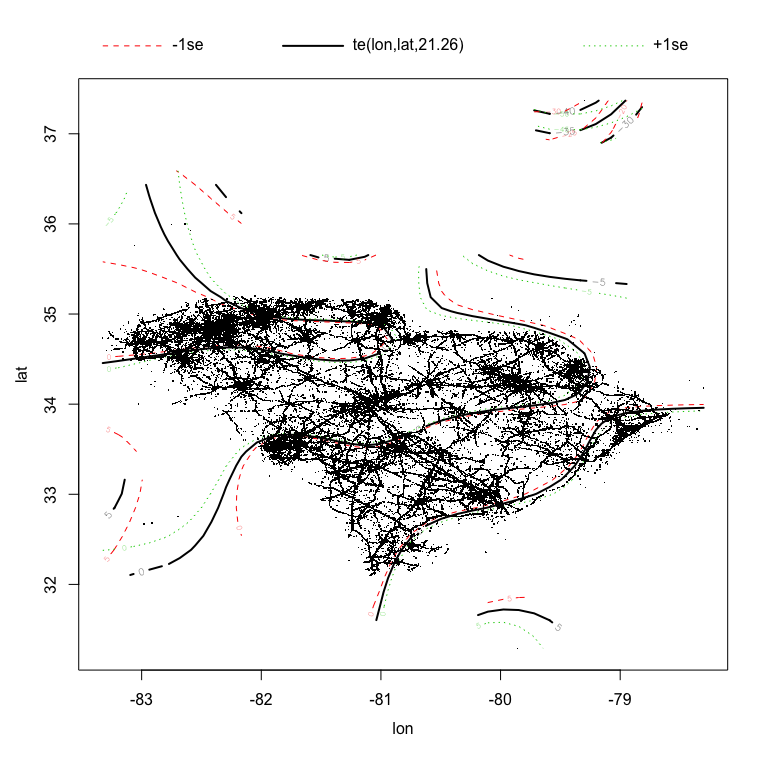
\includegraphics[scale=0.2]{figures/spatialSmooth}
\end{figure}

\end{multicols}
\end{frame}

\begin{frame}
\frametitle{GAM: Parameter Intuition}

\small{
\begin{align*}
 f(x)&=\sum \limits_{i=1}^q a_i(x) \alpha_k\\
f(x,z)&= \sum \beta_i(z) a_i(x) = \sum_i \sum_j \beta_{ij} b_j(z) a_i(x) \\
\end{align*}}
\vspace{-.3in}
\begin{figure}
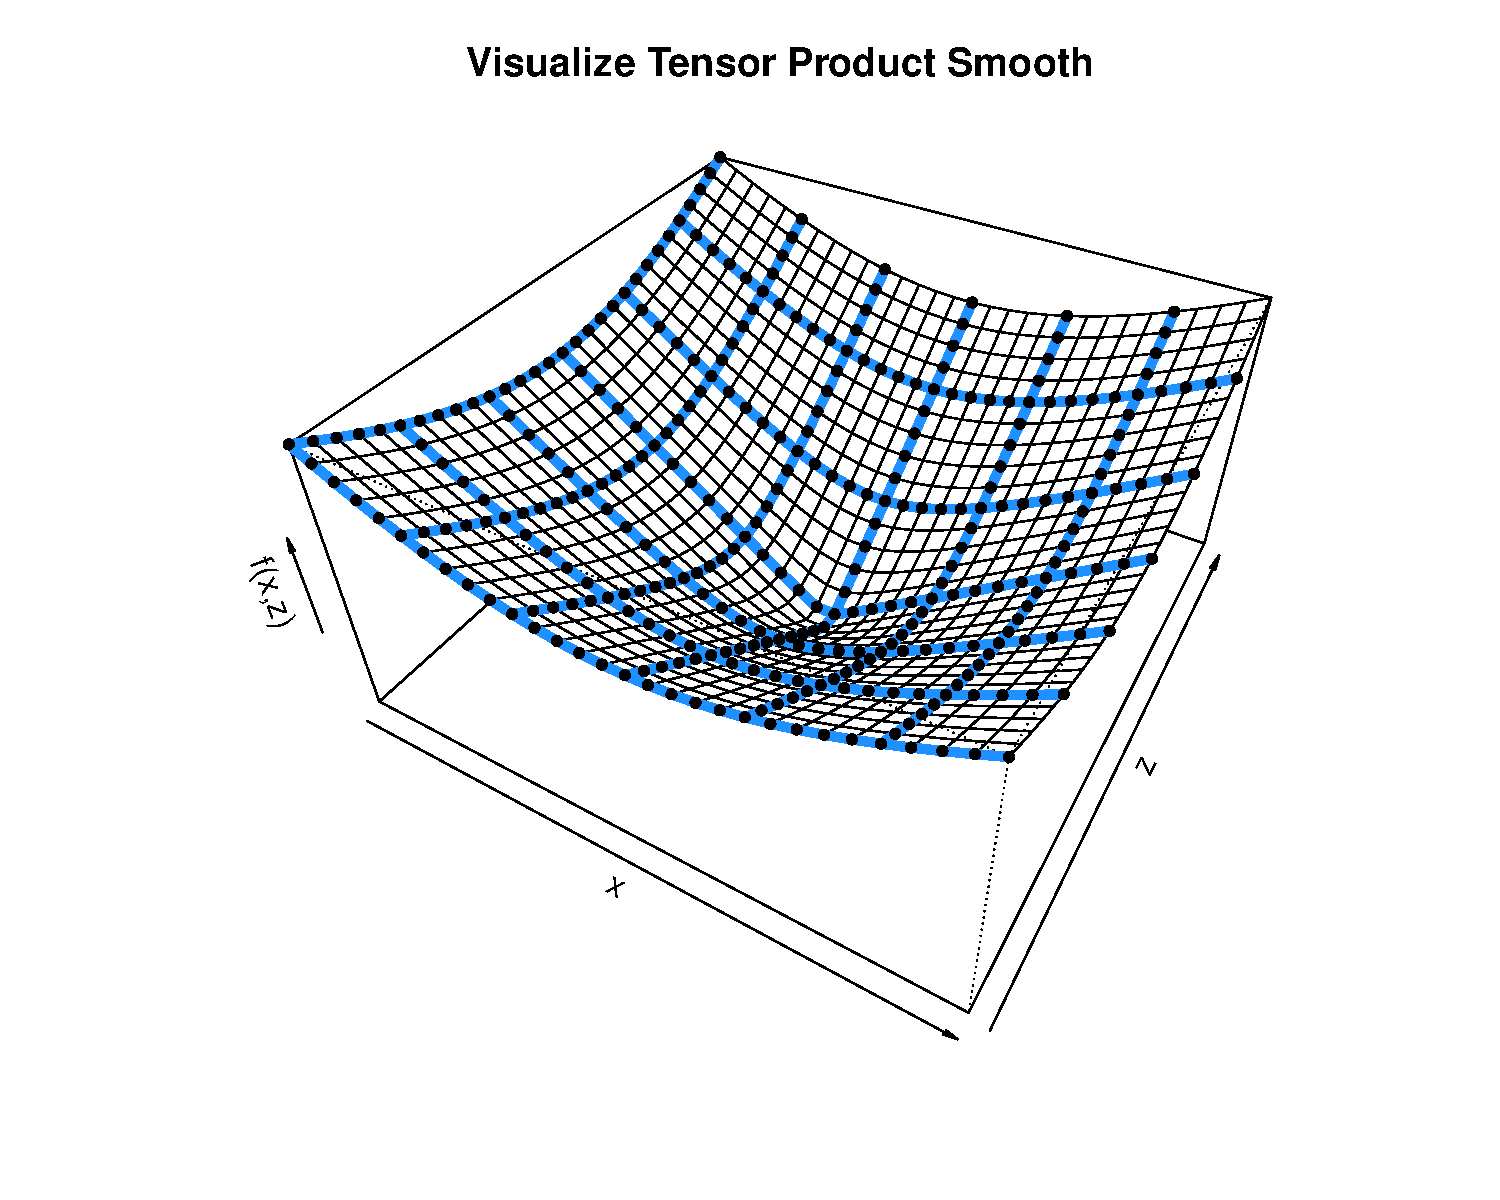
\includegraphics[scale=.25]{figures/tensorProductViz}

\end{figure}

\end{frame}

\begin{frame}
\frametitle{Spatial Predictions}

\begin{figure}
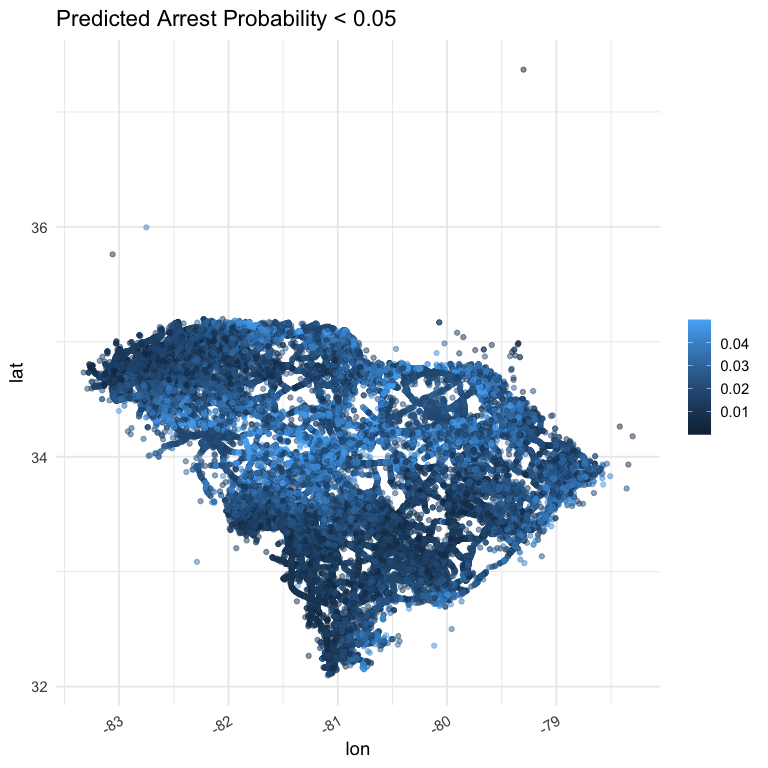
\includegraphics[scale=.2]{figures/spatialPredLow}
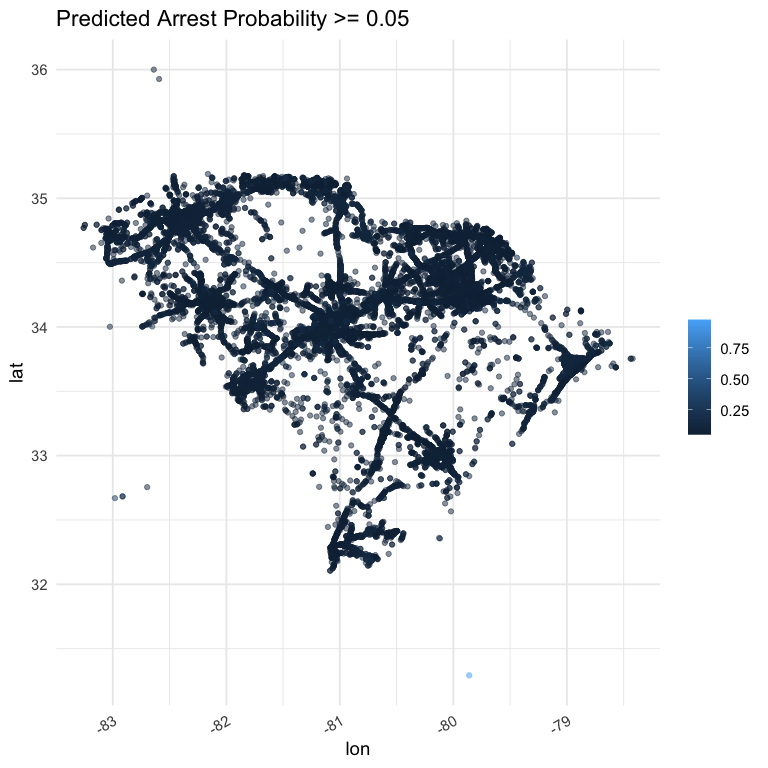
\includegraphics[scale=.2]{figures/spatialPredHigh}
\end{figure}

\end{frame}

\begin{frame}
\frametitle{Decomposition}



$$g(\text{arrest}) \sim \beta_{driverRace} +  \beta_{gender} + f_1(\text{age}) +\beta_{isPostPolicy}+ \beta_{driverRace, isPostPolicy}+$$
$$ ti(\text{lon}) + ti(\text{lat})+ ti(\text{lon, lat})$$



\begin{figure}
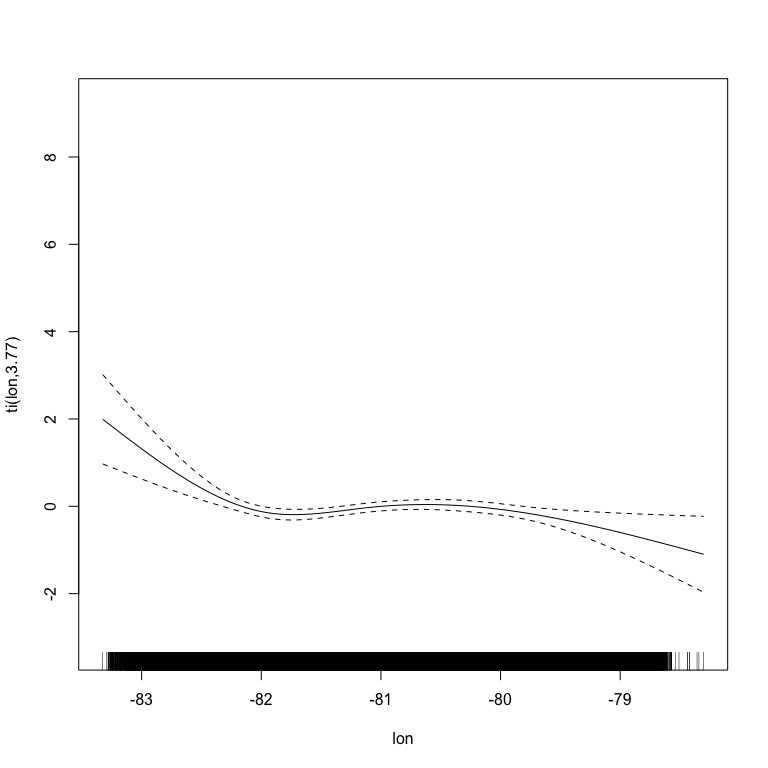
\includegraphics[scale=.2]{figures/lon}
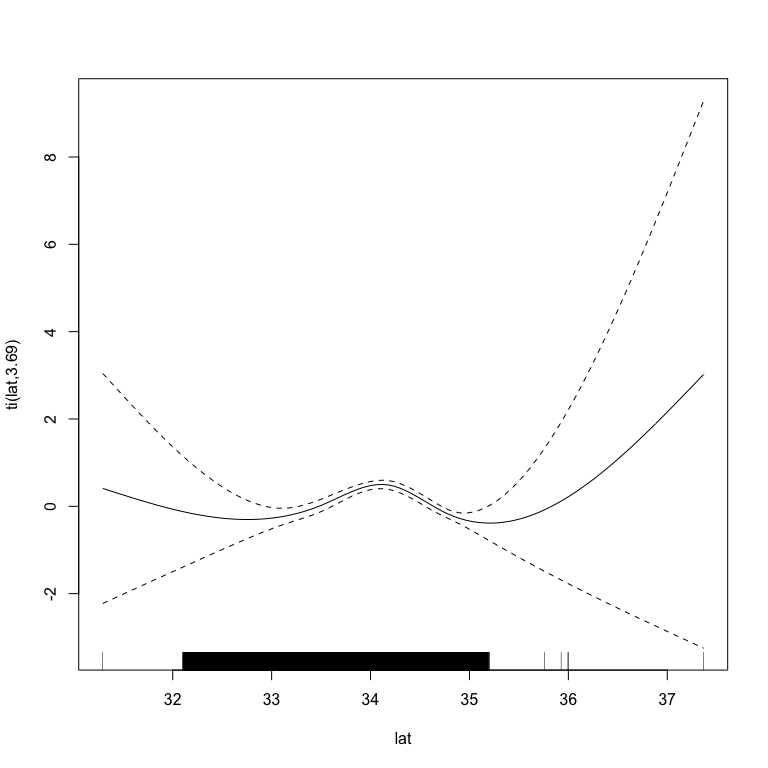
\includegraphics[scale=.2]{figures/lat}

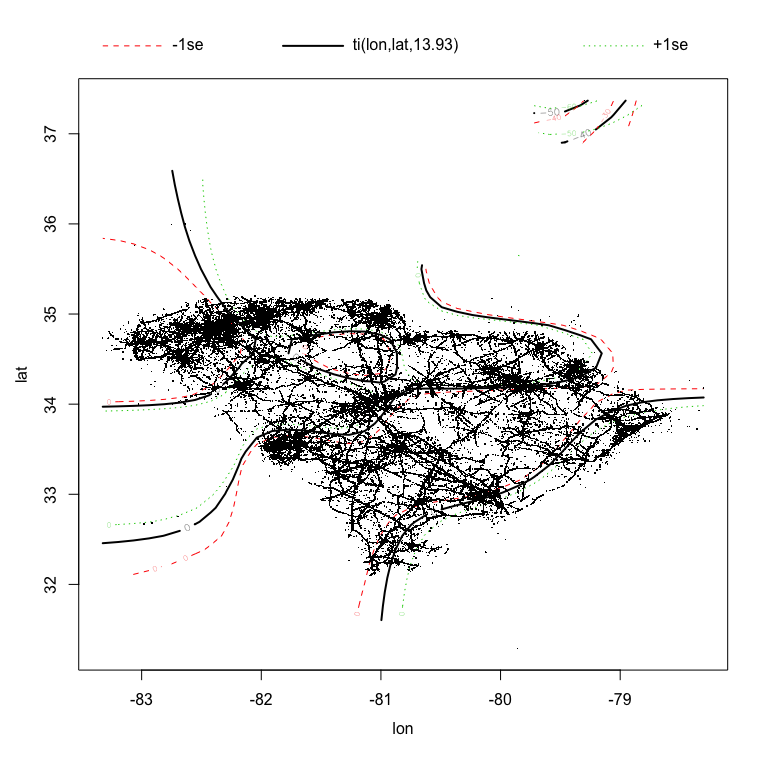
\includegraphics[scale=.2]{figures/lonlat}
\end{figure}

\end{frame}

\begin{frame}
\frametitle{Decomposition}

\begin{multicols}{2}

\begin{figure}
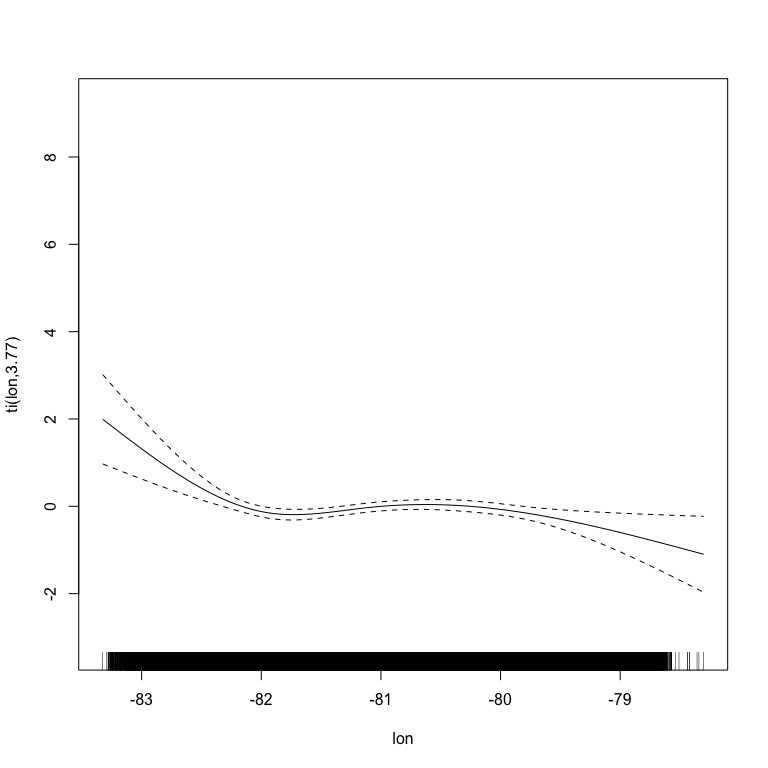
\includegraphics[scale=.1]{figures/lon}

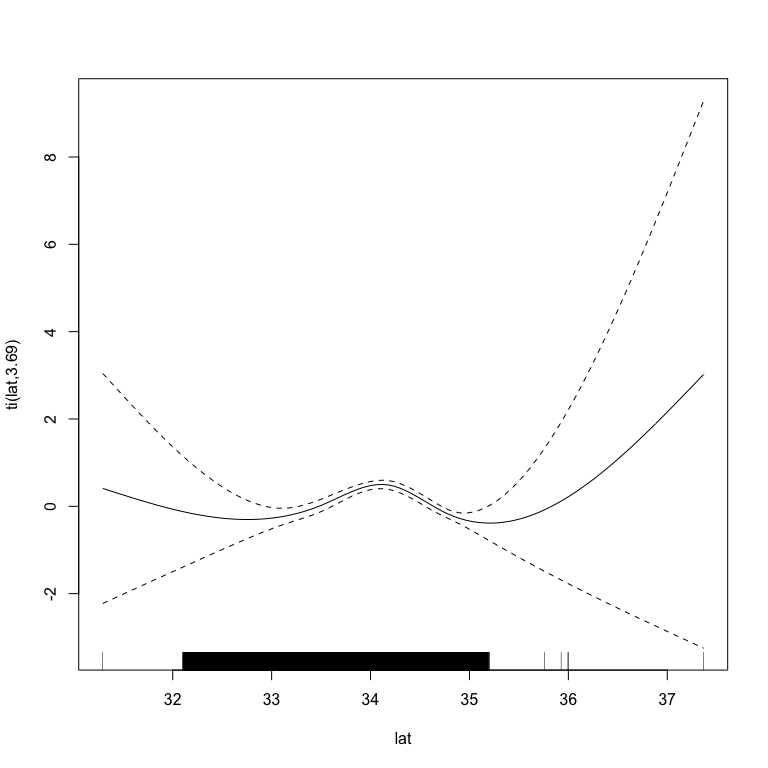
\includegraphics[scale=.1]{figures/lat}
\end{figure}

\columnbreak

\begin{figure}
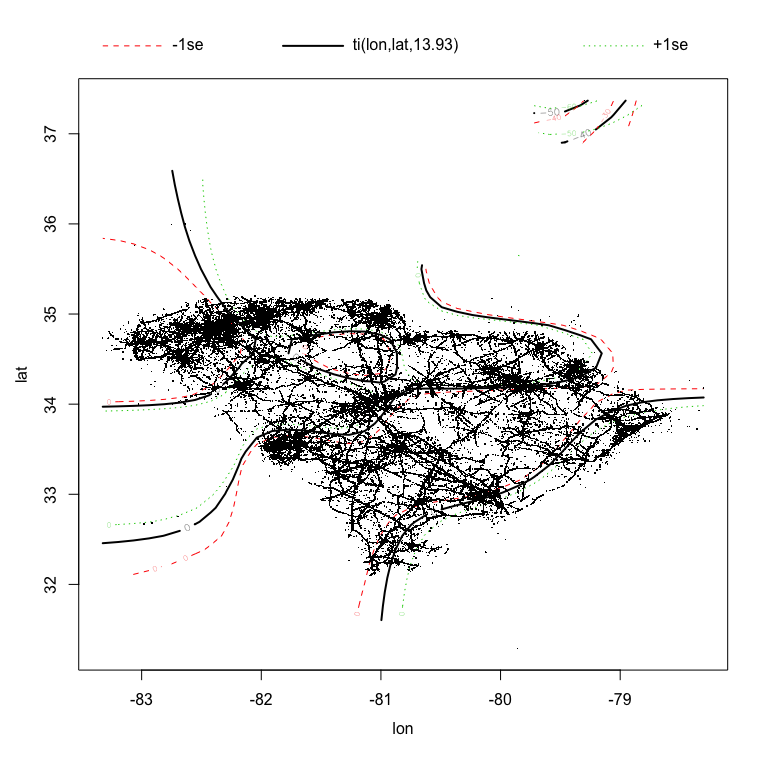
\includegraphics[scale=.2]{figures/lonlat}
\end{figure}

\end{multicols}


\end{frame}

\begin{frame}
\frametitle{More Resources}
\begin{itemize}
\item Simon N. Wood. \textit{Generalized Additive Models: An Introduction with R.} Chapman and Hall/CRC, 2017.
\item \url{https://noamross.github.io/gams-in-r-course/}
\item \url{http://environmentalcomputing.net/intro-to-gams/}
\item \url{https://fromthebottomoftheheap.net/2021/02/02/random-effects-in-gams/}
\item \url{https://www.tjmahr.com/random-effects-penalized-splines-same-thing/}
\item many, many more...
\end{itemize}
\end{frame}

\begin{frame}
\LARGE

\begin{center}
\frametitle{Time to GAM-ify your own work?}
Questions?

\vspace{.2in}

sstoudt@smith.edu

\vspace{.2in}

@sastoudt

\end{center}
\end{frame}

\begin{frame}
\frametitle{I'll leave you with some other Wiggles...}

\begin{figure}

\includegraphics[scale=.4]{figures/wiggles}
\caption{\url{https://www.youtube.com/watch?v=a13WnqsRc5g }}
\end{figure}

\end{frame}


% end with some other wiggles 
%https://www.youtube.com/watch?v=a13WnqsRc5g 


\end{document} 